\documentclass[paper=a4, fontsize=18pt]{article} % A4 paper and 11pt font size
\usepackage{lmodern}
\usepackage[T1]{fontenc} % Use 8-bit encoding that has 256 glyphs
\usepackage{graphicx}
\usepackage{epstopdf}
\usepackage{subfigure}
%\usepackage{fourier} % Use the Adobe Utopia font for the document - comment this line to return to the LaTeX default
\usepackage[english]{babel} % English language/hyphenation
\usepackage{amsmath,amsfonts,amsthm} % Math packages
\usepackage[linesnumbered,ruled,vlined]{algorithm2e}
\usepackage{lipsum} % Used for inserting dummy 'Lorem ipsum' text into the template
\usepackage{sectsty} % Allows customizing section commands
\usepackage{hyperref}
%\allsectionsfont{\centering \normalfont\scshape} % Make all sections centered, the default font and small caps

\usepackage{fancyhdr} % Custom headers and footers
\usepackage{multirow}
%\usepackage{multicolumn}
\pagestyle{fancyplain} % Makes all pages in the document conform to the custom headers and footers
\fancyhead{} % No page header - if you want one, create it in the same way as the footers below
\fancyfoot[L]{} % Empty left footer
\fancyfoot[C]{} % Empty center footer
\fancyfoot[R]{\thepage} % Page numbering for right footer
\renewcommand{\headrulewidth}{0pt} % Remove header underlines
\renewcommand{\footrulewidth}{0pt} % Remove footer underlines
\setlength{\headheight}{13.6pt} % Customize the height of the header
\setlength{\parskip}{0.5\baselineskip}

\numberwithin{equation}{section} % Number equations within sections (i.e. 1.1, 1.2, 2.1, 2.2 instead of 1, 2, 3, 4)
\numberwithin{figure}{section} % Number figures within sections (i.e. 1.1, 1.2, 2.1, 2.2 instead of 1, 2, 3, 4)
\numberwithin{table}{section} % Number tables within sections (i.e. 1.1, 1.2, 2.1, 2.2 instead of 1, 2, 3, 4)

\newcommand{\mM}{\mathcal{M}}
\newcommand{\mL}{\mathcal{L}}
\newcommand{\mB}{\mathcal{B}}
\newcommand{\mT}{\mathcal{T}}
\newcommand{\mS}{\mathcal{S}}
\newcommand{\mP}{\mathcal{P}}
\newcommand{\bH}{\mathbb{H}}

\setlength\parindent{0pt} % Removes all indentation from paragraphs - comment this line for an assignment with lots of text

\graphicspath{{pic/}}

%----------------------------------------------------------------------------------------
%	TITLE SECTION
%----------------------------------------------------------------------------------------
\newtheorem{definition}{Definition}{\itshape}{\rmfamily}
\newtheorem{theorem}{Theorem}{\itshape}{\rmfamily}
\newtheorem{corollary}{Corollary}{\itshape}{\rmfamily}
\newtheorem{example}{Example}{\itshape}{\rmfamily}
\newtheorem{proposition}{Proposition}{\itshape}{\rmfamily}
\newcommand{\horrule}[1]{\rule{\linewidth}{#1}} % Create horizontal rule command with 1 argument of height

\title{	
\normalfont \normalsize
\horrule{0.5pt} \\[0.4cm] % Thin top horizontal rule
\huge Survey of Intelligent Chatbots and Conversational Interfaces \\ % The assignment title
\horrule{2pt} \\[0.5cm] % Thick bottom horizontal rule
}
\hypersetup{hidelinks}

\author{}


\begin{document}

\maketitle
\tableofcontents

\section{Overview}

\textbf{\emph{Chatbots}}, also known as \emph{conversational agents}, \emph{dialogue systems}, and sometimes \emph{chatterbots}, can be divided into \emph{goal-oriented systems} and \emph{non-goal-driven systems}. A typical system architecture is shown in Figure \ref{system architecture}. It consists of six components: \emph{automatic speech recognition (ASR)}, \emph{natural language understanding (NLU)}, \emph{dialogue manager (DM)}, \emph{task manager (TM)}, \emph{natural language generation (NLG)}, and \emph{text-to-speech synthesis (TTS)} \cite{Jurafsky2006}.

\begin{figure}[htbp]
  \centering
  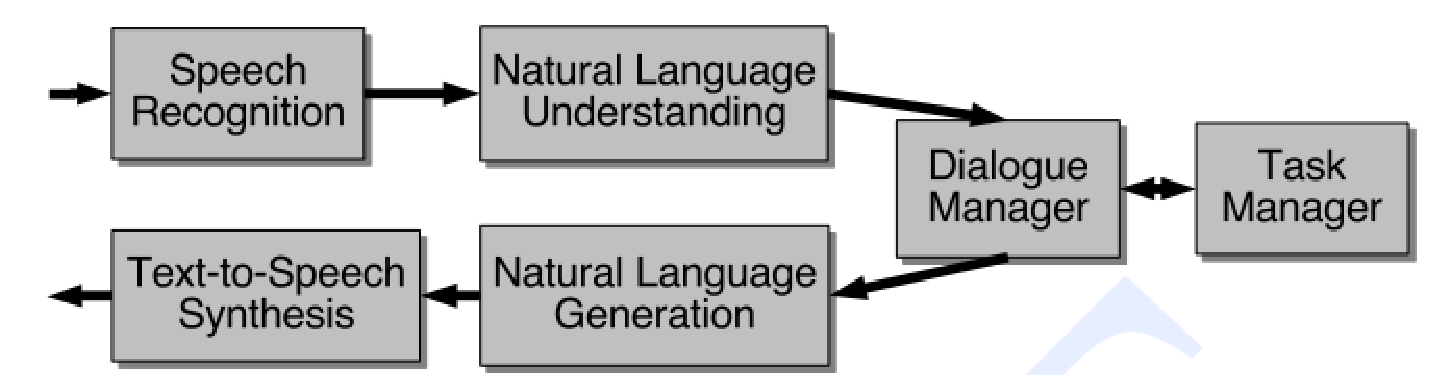
\includegraphics[width=\linewidth]{system_architecture}
  \caption{An example of system architecture}
	\label{system architecture}
\end{figure}

The following sections of this survey paper are organized as follows: From Section \ref{Automatic Speech Recognition} to Section \ref{Text-to-speech Synthesis}, we will introduce the components of goal-driven systems in further detail. Since the TM (task manager) component depends on the specific task at hand, we do not provide any paper about it. We start with each section a brief summary of the goal of the component, and then present some related previous work. Finally in Section \ref{Non-goal-driven Systems}, we present some papers about non-goal-driven systems.

\section{Automatic Speech Recognition} \label{Automatic Speech Recognition}

The \emph{ASR (automatic speech recognition)} component takes audio input, generally from a telephone, or from a PDA of desktop microphone, and returns a transcribed string of words \cite{Jurafsky2006}.

Most of the successful ASR systems are based on the mathematical foundation of \emph{hidden Markov models (HMM)}. So we begin this section with presenting a tutorial paper of this subject \cite{Rabiner1989A}. The most successful ASR approach has been \emph{HMM-GMM (Gaussian mixture model)}, until the recent emergence of the \emph{HMM-DNN (deep neural network)} approach. The next two sections present two selected papers of the HMM-DNN method \cite{Hinton2012Deep,Graves2013Speech}. The field of ASR has been investigated for many decades, and lots open-source systems are available. Among the many choices, Kaldi \cite{DanielPovey2014} is drawing more and more attentions due to its perfect support for the DNN techniques. In the fourth and the fifth summaries \cite{Mohri2000,Ljolje1999}, we discuss two important topics that are widely applied in the Kaldi system, namely the \emph{weighted finite-state transducer (WFST)} and \emph{lattice}. Finally, we briefly introduce a speaker adaption technique \cite{Leggetter1995}.

\subsection{A tutorial on hidden Markov models and selected applications in speech recognition \cite{Rabiner1989A}}

This paper is a very classic and comprehensive tutorial on \emph{Hidden Markov Models (HMMs)}. Although HMMs is not among the deep learning approaches that emerged in recent years, the concepts behind HMMs are closely related to that of the \emph{Recurrent Neural Networks (RNNs)}.

\begin{figure}[htbp]
  \centering
  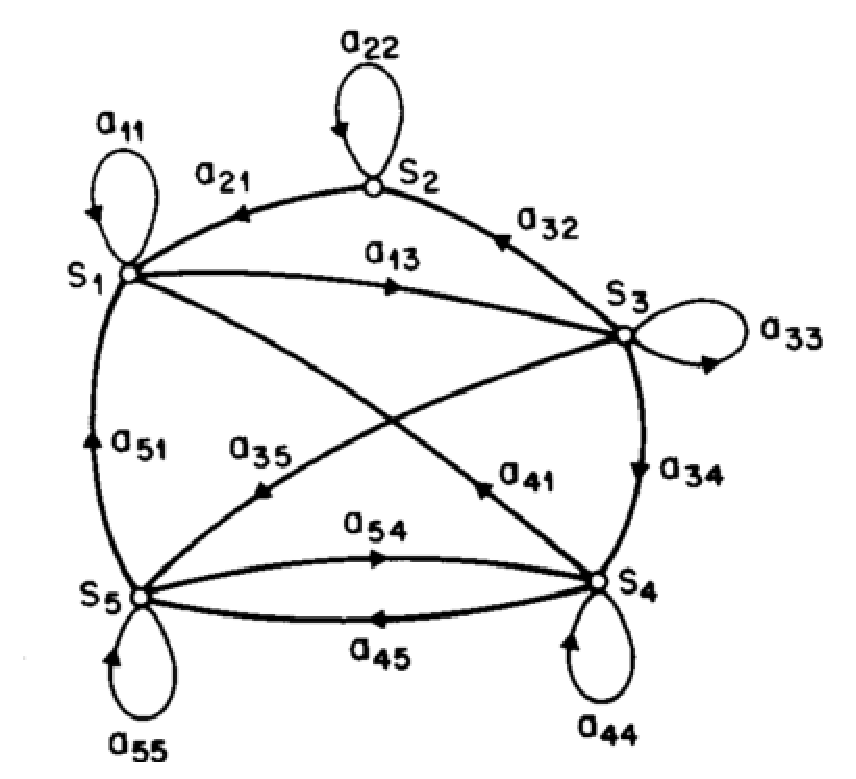
\includegraphics[width=.6\linewidth]{8_29_HMM_chain}\\
  \caption{A Markov chain with 5 states}\label{fig:chain}
\end{figure}

In the discrete Markov processes (without hidden states), a system at any time is described as being in one of a set of distinct state (cf. Figure \ref{fig:chain}). A full probabilistic description of the above system would require specification of the current state, as well as all the predecessor states. For the special case of a discrete, first order, Markov chain, it is assumed that the probabilistic description only depends on the current state and its immediate predecessor. This stochastic process is also called an observable Markov model, since the output of the process is the set of states at each instant of time, where each state corresponds to a physical (observable) event.

HMMs extend the concept to include the case where the observation is a probabilistic function of the hidden states, i.e., the resulting model is a doubly embedded stochastic process with an underlying stochastic process that is not observable, but can only be observed through another set of stochastic processed that produce the observations.

It would be better to explain the concept with the following example. Suppose on the other side of the curtain a person is performing a coin tossing experiment. That person will not tell you anything about what he is doing exactly (he may be tossing 2 or 3 different coins with different biased coins); he will only tell you the result of each coin flip (the observation).

\begin{figure}[htbp]
  \centering
  \subfigure{
    \label{fig:topka} %% label for first subfigure
    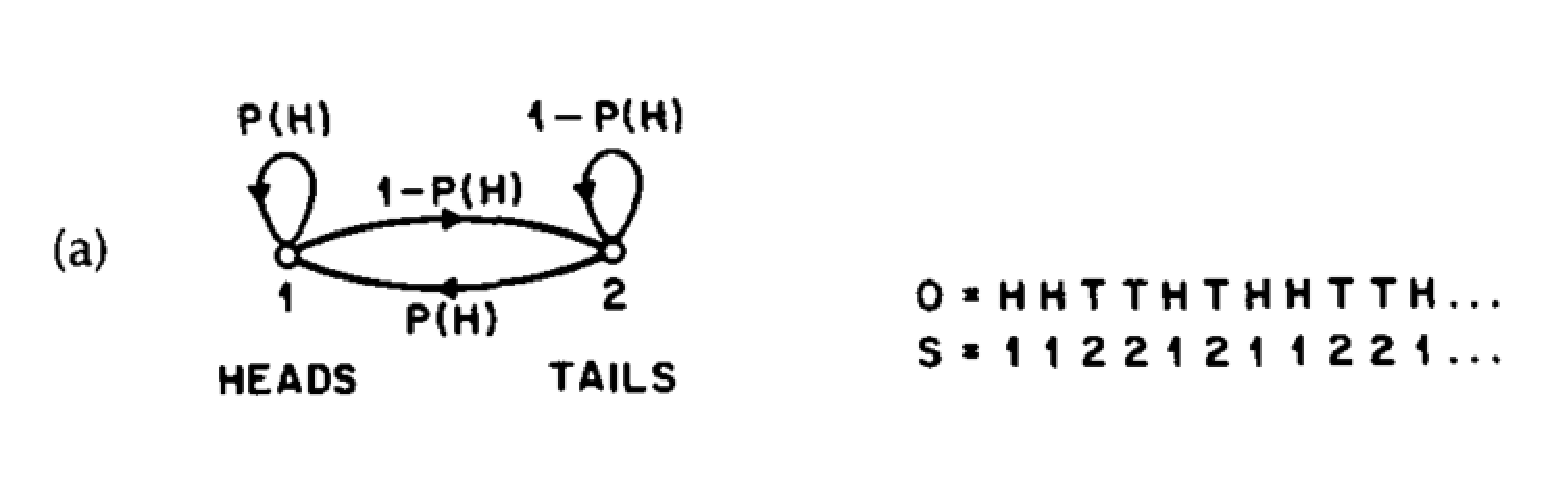
\includegraphics[width=2.2in]{8_29_HMM_coinA}}
  \subfigure{
    \label{fig:topkb} %% label for second subfigure
    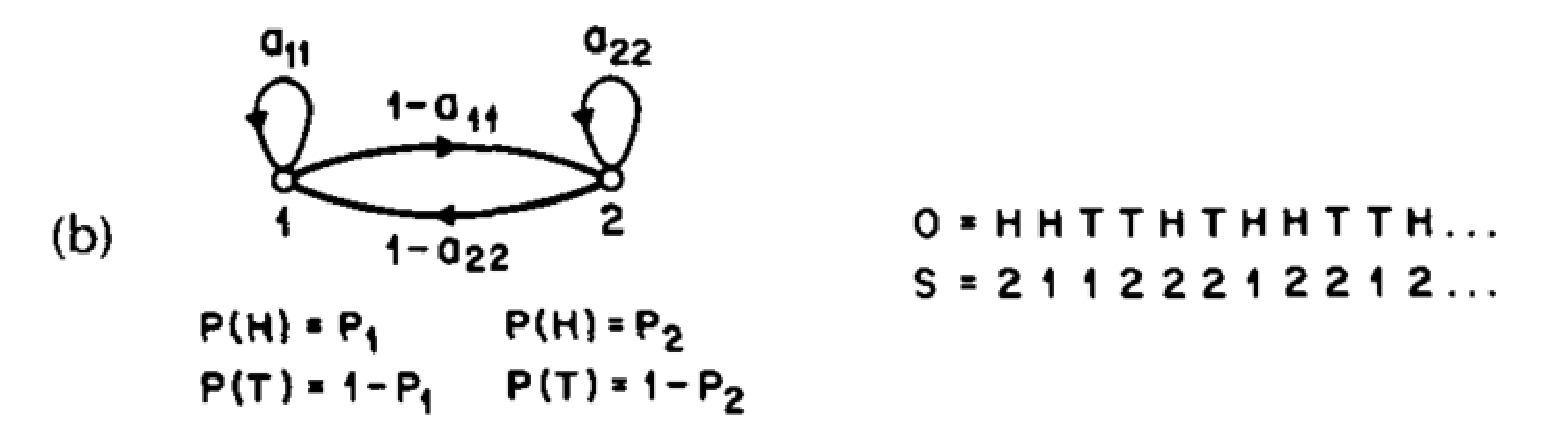
\includegraphics[width=2.2in]{8_29_HMM_coinB}}
  \subfigure{
    \label{fig:topkb} %% label for second subfigure
    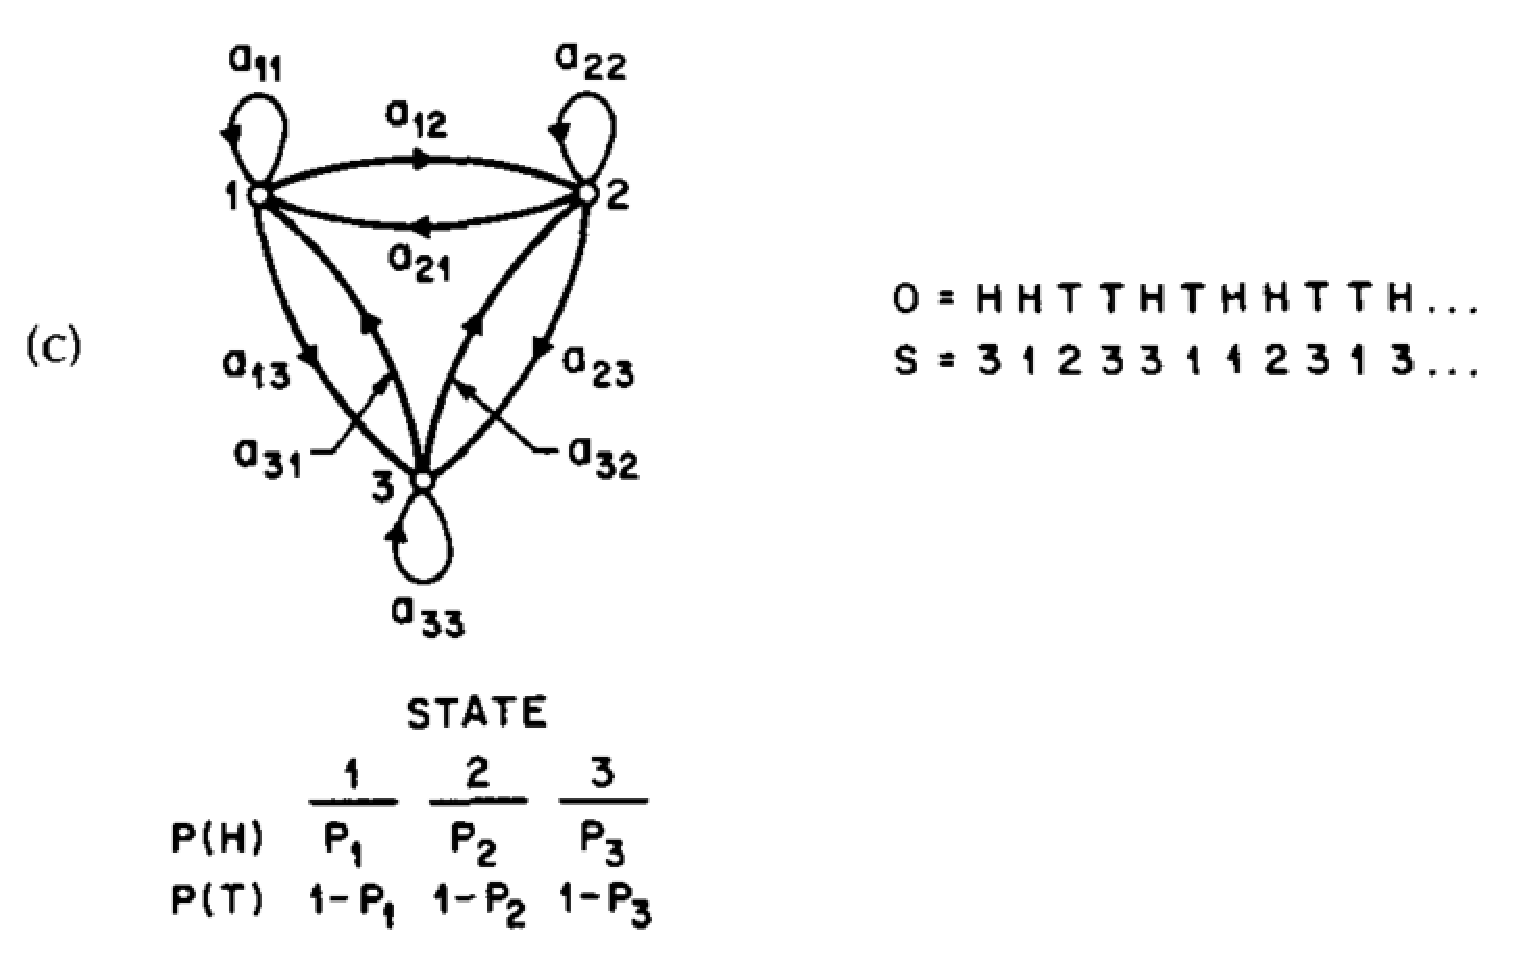
\includegraphics[width=2.2in]{8_29_HMM_coinC}}
  \caption{Three possible Markov models that can account for the results of hidden coin tossing experiments}\label{fig:coin}
\end{figure}

One possible choice would be to assume that only a single coin was being tossed. In this case the situation could be model with a 2-state (fully observable) model where each state corresponds to a side of the coin (cf. Figure \ref{fig:coin} (a)). We can also assume that two different biased coins were being tossed, and use the HMM in Figure \ref{fig:coin} (b) to describe this situation. Here each state corresponds to a different coin. Each state is characterized by a probability distribution of heads and tails, and transitions between states are characterized by a state transition matrix. We could further assume that there are 3 different coins, and model the system as a HMM with 3 hidden states (cf. Figure \ref{fig:coin} (c)).

An HMM is mathematically characterized by the following parameters: 1) $N$, the number of states in the model; 2) $M$, the number of distinct observation symbols; 3) The state transition probability distribution $A=\{a_{ij}\}$; 4) The observation symbol probability distribution in state $j$, $B = \{b_j(k)\}$; 5) The initial state distribution $\pi$. The paper uses the compact notation $\lambda = (A, B, \pi)$ to indicate the complete parameter set of the models.

There are three basic problems for HMMs: 1) How to efficiently compute $P(O| \lambda)$, the probability of the observation sequence given the model; 2) Given the observation sequence $O$ and the model $\lambda$, how to choose a corresponding state sequence $Q$ that is optimal; 3) How to adjust (or train) the parameters in $\lambda$ to maximize $P(O| \lambda)$.

The paper shows that all the three problems can be solved by the \emph{forward-backward procedure}. The basic idea of the forward-backward procedure is to apply the technique of dynamic programming. It introduces a forward variable $\alpha_t(i)$, which is probability of the partial observation sequence $O_1, ..., O_t$ (until time $t$) and state $S_i$ at time $t$. It shows how $\alpha_{t+1}(i)$ can be computed based on $\alpha_t(i)$ (the idea of dynamic programming). Similarly, a backward variable $\beta_t(i)$ is defined as the probability of the partial observation sequence from $t+1$ to the end. Finally, all the three problems can be solve by using the forward and backward variables.

In the remaining parts of the paper, it introduces various types of HMMs that have been previously studied (for example HMMs whose states are not fully connected). It also discusses the issues that arise in implementations, such as initial parameter estimates, model size, missing data, etc. Finally it describes some successful applications of HMMs in the field of speech recognizer.

\subsection{Deep Neural Networks for Acoustic Modeling in Speech Recognition \cite{Hinton2012Deep}}

This paper provides an overview of the progress of acoustic modeling by \emph{deep neural networks (DNNs)}. It also presents the shared view of four research groups (groups at the University of Toronto, Microsoft Research, Google, and IBM Research) that have had recent successes in using this technique.

The goal of the acoustic modeling in this paper is to determine how well each state of a \emph{hidden Markov model (HMM)} fits a frame or a short window of frames of coefficients that represents the acoustic input $p(HMMstate | AcousticInput)$. So the produced acoustic model is combined with the classic HMM to form the final hybrid \emph{automatic speech recognition (ASR)} system.

In modern ASR systems, the acoustic input is typically represented by concatenating \emph{Mel-frequency cepstral coefficients (MFCCs)} or \emph{perceptual linear predictive coefficients (PLPs)}, computed from the raw waveform and their first- and second-order temporal differences. The preprocessing techniques are designed to discard the large amount of information in waveforms that is considered to be irrelevant for discrimination.

The DNN approach for acoustic modeling has two key stages. In the first stage, layers of feature detectors are initialized, one layer at a time, by fitting a stack of generative models. In the second stage, each generative model in the stack is used to initialize one layer of hidden units in a DNN. Finally the whole network is then discriminatively fine-tuned to predict the target HMM states.

The idea behind the first stage is generative pretraining: it finds a region of the weight-space that allows the discriminative fine-tuning to make rapid progress, and it also significantly reduces overfitting. The generative model in DNN approaches uses a set of parameters, $W$, to define the joint probability of a vector of observable variables $v$, and a vector of latent variables $h$, via an energy function $E$:
$$p(v,h; W) = \frac{1}{Z} e^{-E(v,h; W)}, Z = \sum_{v', h'} e^{-E(v', h'; W)}.$$
In the classic \emph{restricted Boltzmann machine (RBM)} which consists of a layer of stochastic binary visible units and a layer of stochastic binary hidden units, the energy function is defined to be:
$$E(v,h) = -\sum_{i \in  visible} a_i v_u - \sum_{j \in hidden} b_j h_j - \sum_{i,j} v_i h_i w_{ij},$$
where $v_i, h_j$ are the binary states of visible unit $i$ and hidden unit $j$, $a_i, b_j$ are their biases, and $w_{ij}$ is the weight between them. The training of a RBM can be achieved by the \emph{contrastive divergence (CD)} algorithm.

After training an RBM on the data, the inferred states of the hidden units can be used as data for training another RBM that learns to model the dependencies between the hidden units of the first RBM. This can be repeated many times to produce many layers of nonlinear feature detectors, which is called a \emph{deep believe network (DBN)}.

\begin{figure}[htbp]
  \centering
  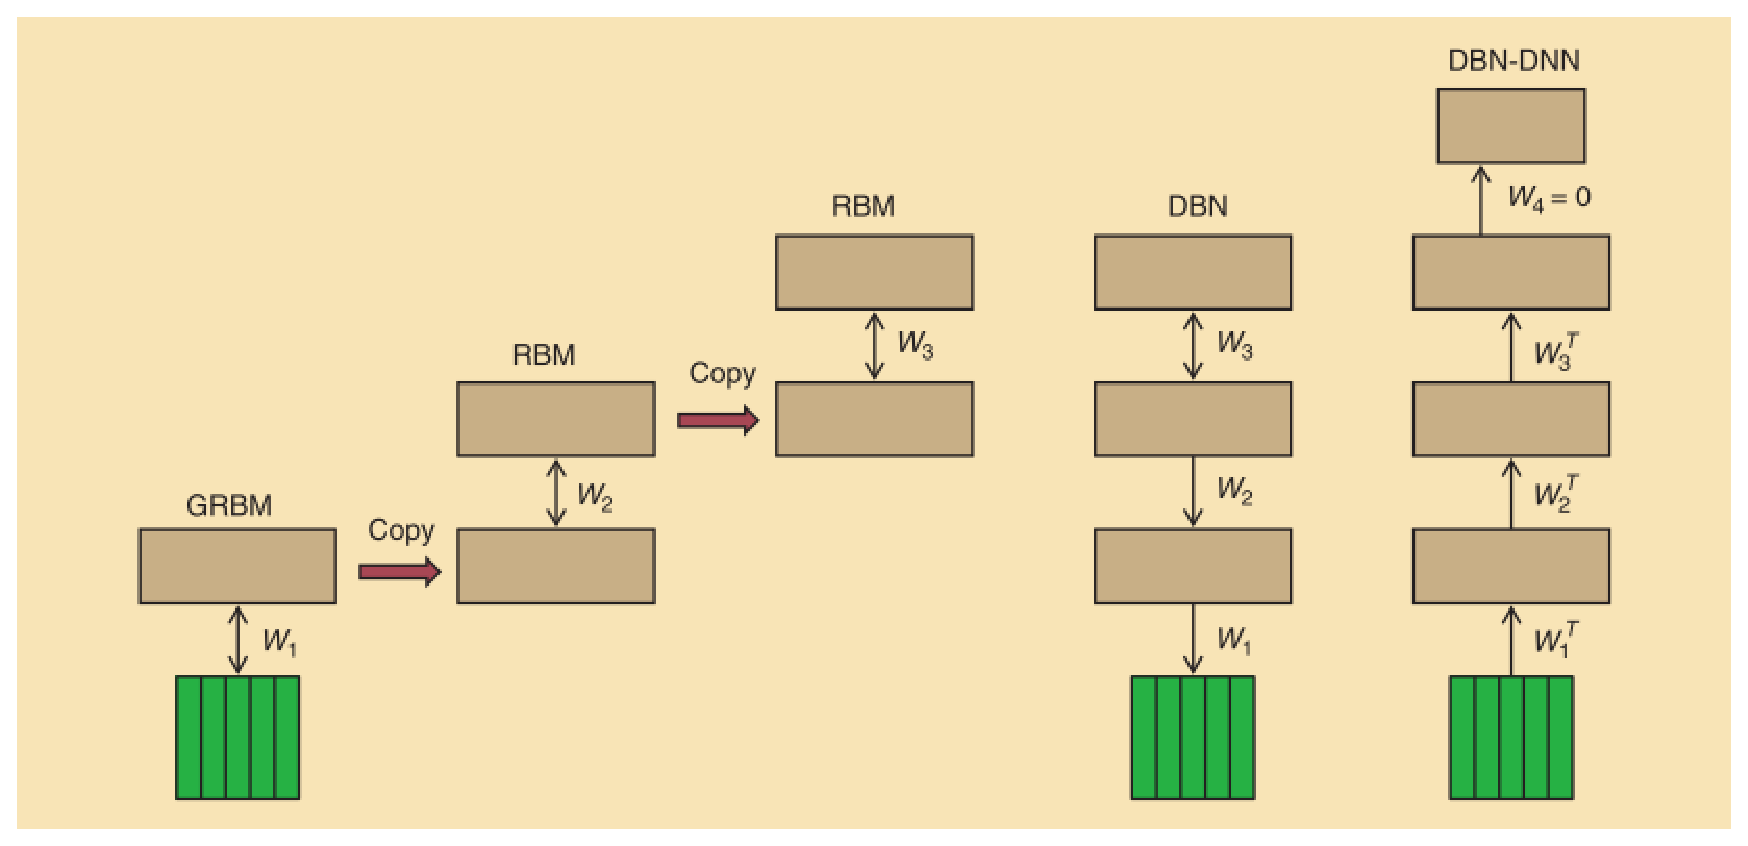
\includegraphics[width=.9\linewidth]{10_17_HMM_DNN}\\
  \caption{Illustration of the DNN training process}\label{fig:HMM_DNN}
\end{figure}

After learning a DBN by training a stack of RBMs, the generative weights in the reverse direction are used as the initialization of a feedforward DNN. It then adds a final softmax layer and trains the whole DNN discriminatively. The whole architecture is illustrated in Figure \ref{fig:HMM_DNN}: 1) A \emph{Gaussian RBM (GRBM)} is trained to model real-valued acoustic coefficients. Then the hidden states of the GRBM are used as data for training the next RBM. 2) This is repeated to create as many hidden layers as desired. 3) Finally, a pretrained DBN-DNN is created by adding a softmax output layer that predicts the hidden state of the HMM.

In the experimental study, the paper reports the results on the TIMIT benchmark and on several large-vocabulary speech recognition datasets. For example in the Bing-voice-search speech recognition task, the best DNN-HMM acoustic model achieves a sentence accuracy of 69.6\% on the test set, compared with 63.8\% for a strong HMM baseline method.

\subsection{Speech Recognition With Deep Recurrent Neural Networks \cite{Graves2013Speech}}

End-to-end training methods such as \emph{Connectionist Temporal Classification (CTC)} make it possible to train RNNs for sequence labelling problems where the input-output alignment is unknown. However, RNN performance in speech recognition has so far been disappointing. This paper investigates deep recurrent neural networks on the ASR task, and shows that the method achieves a test set error of 17.7\% on the TIMIT phoneme recognition benchmark, which is the best recorded score.

The goal of this paper is to investigate whether RNNs could benefit from depth in space - that is, stacking multiple recurrent hidden layers on top of each other.

\begin{figure}[htbp]
  \centering
  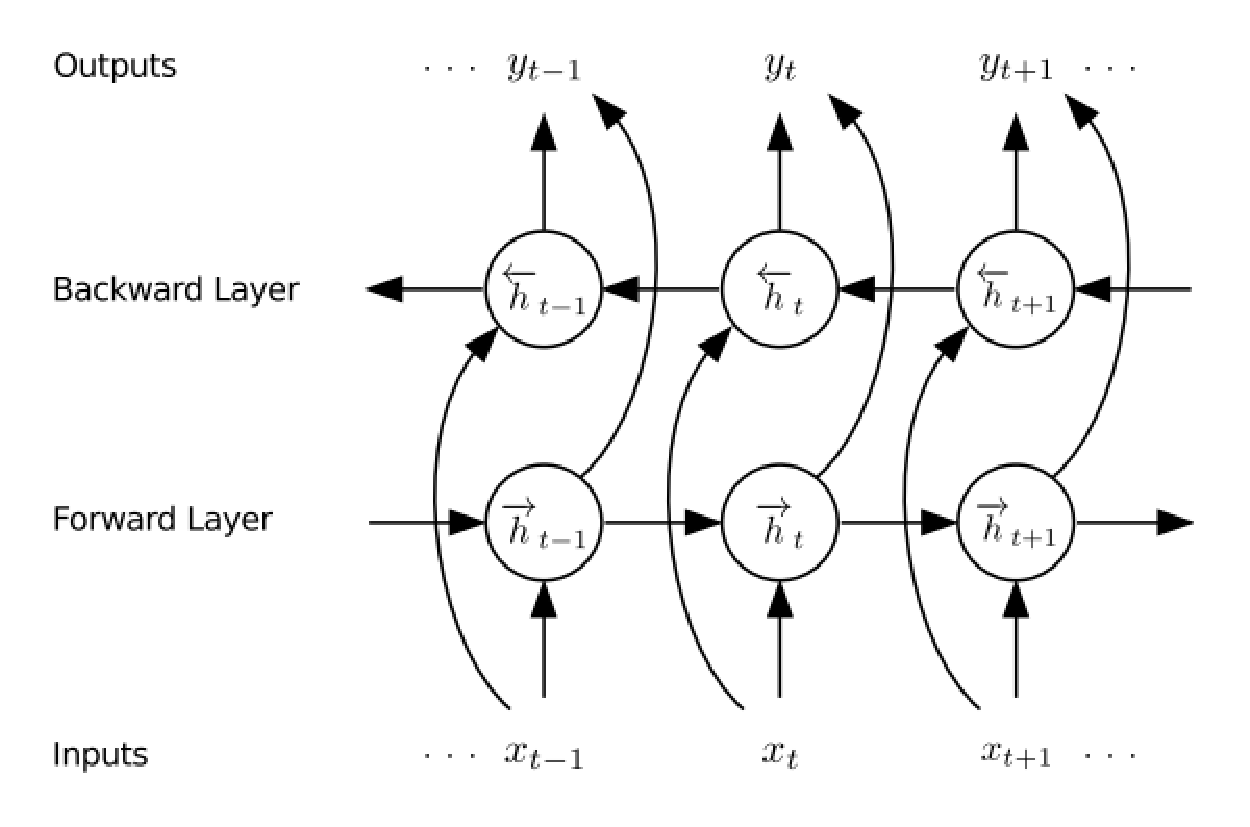
\includegraphics[width=.5\linewidth]{10_17_ASR_RNN}\\
  \caption{Bidirectional RNN}\label{fig:ASR_RNN}
\end{figure}

The concepts of RNN and \emph{long short-term memory (LSTM)} unit have been discussed in previous paper summaries. The basic architecture in this paper is based on the \emph{bidirectional RNNs (BRNNs)}. The basic idea of BRNN is to process the data in both directions (forward and backward) with two separate hidden layers. Figure \ref{fig:ASR_RNN} shows an example of a BRNN model that computes the forward hidden sequence $\stackrel{\rightarrow}{h}$, the backward hidden sequence $\stackrel{\leftarrow}{h}$, and the output sequence $y$. Combining BRNNs with LSTM gives \emph{bidirectional LSTM}.

In the RNN training, the RNNs map directly from acoustic to phonetic sequences. The paper presents two ways to define the output distribution and hence train the network.

The first method is called Connectionist Temporal Classification, which uses a softmax layer to define a separate output distribution $Pr(k|t)$ at every step $t$ along the input sequence. CTC then uses a \emph{forward-backward algorithm} to sum over all possible alignments and determine the normalised probability $Pr(z|x)$ of the target sequence.

The second method is based on the \emph{RNN transducer} technique, which combines a CTC-like network with a separate RNN that predicts each phoneme given the previous ones, thereby yielding a jointly trained acoustic and language model. The basic idea of RNN transducer is to determine a separate distribution $Pr(k | t, u)$ for every combination of input timestep $t$ and output timestep $u$. Specifically, $Pr(k | t, u)$ is defined by taking an `acoustic' distribution $Pr(k | t)$ from the CTC network, a `linguistic' distribution $Pr(k | u)$ from the prediction network, then multiplying them together and renormalising.

In the experimental study, the proposed model is evaluated on the TIMIT corpus. It is reported that the \emph{phoneme error rate (PER)} on the core test set is 17.7\%, which is the best result known to the authors.

Remark: I have also consider the possibility of applying RNNs on the ASR task. This paper shows that this is indeed a promising approach. Compared to the HMM-based or hybrid methods, the approach of this paper is simpler and more elegant - it can jointly train the acoustic and language models in an end-to-end fashion. However, this method is still not very mature, since the TIMIT benchmark is restricted in size. As mentioned by the authors, a possible future work is to extend the system to large vocabulary speech recognition.

\subsection{Speech Recognition with Weighted Finite-State Transducers \cite{Mohri2000}}

This paper describes a general representation and algorithmic framework for speech recognition based on \emph{weighted finite-state transducers (WFST)}. These transducers provide a common and natural representation for major components of speech recognition systems, including \emph{hidden Markov models (HMMs)}, context-dependency models, pronunciation dictionaries, etc. The paper shows the application of the proposed method to large-vocabulary recognition task.

A \emph{finite-state transducer} is a finite automaton whose state transitions are labeled with both input and output symbols. Therefore, a path through the transducer encodes a mapping from an input symbol sequence, or string, to an output string. A weighted transducer puts weights on transitions in addition. In this paper, weights encode the probabilities that accumulates along the path.

\begin{figure}[h]
  \centering
  % Requires \usepackage{graphicx}
  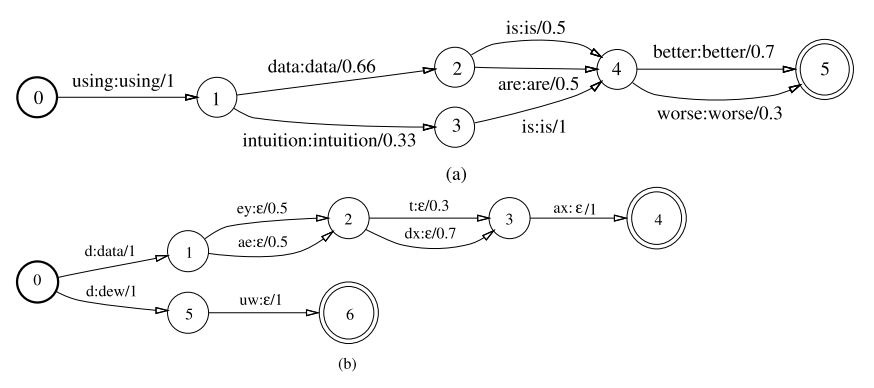
\includegraphics[width=\linewidth]{11_21_WFST.png}\\
  \caption{Examples of weighted finite-state transducer}\label{fig:WFST}
\end{figure}

Figure \ref{fig:WFST} presents a toy language model and a toy pronunciation lexicon as WFSTs. In Figure \ref{fig:WFST}(b), the WFTS maps from phone strings to words in the lexicon, in this example `data' and `dew', with probabilities representing the likelihoods of alternative pronunciations. Similarly, HMM structures can be combined into a single transducer that preserves phone model identity.

The proposed method relies on a common set of weighted transducer operations to combine, optimize, search and prune them. The basic operations \emph{union}, \emph{concatenation}, and \emph{Kleene closure} operations combine transducers in parallel, in series, and with arbitrary repetition, respectively. There are three other key operations that are used in the speech applications:

1) \emph{Composition}: Composition is the transducer operation for combining different levels of representation. For example, a pronunciation lexicon can be composed with a word-level grammar to produce a phone-to-word transducer. In particular, the composition $T = T_1 \circ T_2$ has exactly one path mapping string $u$ to string $w$ for each pair of paths, the first in $T_1$ mapping $u$ to $v$ and the second in $T_2$ mapping $v$ to $w$.

2) \emph{Determinization}: In a deterministic transducer, each state has at most one transition with any given input label and there are no input $\epsilon$-labels. The key advantage of a deterministic transducer is its irredundancy: it contains at most one path matching any given input string, thereby reducing the time and space needed to process the string. The determinization algorithm transforms a non-deterministic WFST into an equivalent deterministic WFST.

3) \emph{Minimization}: Given a deterministic WFST, its size can be reduced by minimization, which can save both space and time. Let the given WFST be denoted as $A$. The minimization algorithm results in a WFST $B$ that is equivalent to $A$, and has the least number of states and the least number of transitions among all deterministic WFSTs equivalent to $A$.

Next we will see how to construct a single recognition transducer that maps from context-dependent phones to a string of words.

Consider the pronunciation lexicon $L$ in Figure \ref{fig:WFST}(b), and the grammar $G$ of Figure \ref{fig:WFST}(a). $L \circ G$ gives a transducer that maps from phones to word strings restricted to the grammar $G$. If we let $C$ represent a transducer from context-dependent phones to context-independent phones, then $C \circ (L \circ G)$ gives a transducer that maps from context-dependent phones (such as triphones) o word strings restricted to the grammar $G$. Finally, the transducer is optimized with determinization and minimization: $N = min(det(C \circ (L \circ G)))$.

In the following sections, the paper introduces the operation algorithms in further details, and reports the experimental results in the large-vocabulary speech recognition task. It is shown that the proposed method can greatly improve the efficiency and save space.

\subsection{Efficient General Lattice Generation and Rescoring \cite{Ljolje1999}}

This paper describes a lattice generation method that produces high-quality lattices with less than 10\% increased computation over standard \emph{Viterbi} decoding. The proposed method is closely related to previous lattice generation methods, but applies to more general network topologies.

\begin{figure}[h]
  \centering
  % Requires \usepackage{graphicx}
  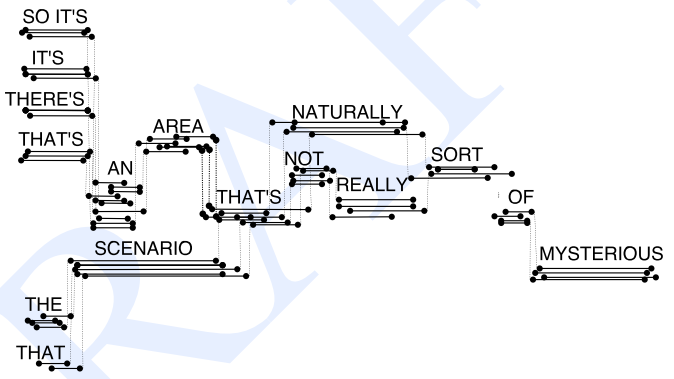
\includegraphics[width=.7\linewidth]{11_21_lattice.png}\\
  \caption{Example of a lattice}\label{fig:lattice}
\end{figure}

In this paper, a \emph{lattice} is defined to be a labeled, weighted, directed acyclic graph in which each complete path represents an alternative transcription hypothesis, weighted by its recognition score for a given utterance. However, it should be noted that there is no generally accepted single definition of lattice. Figure \ref{fig:lattice} shows an example of lattice (figure from Chapter 10 of Speech and Language Processing \cite{Jurafsky2006}).

In this paper, \emph{ASR networks} are represented as \emph{finite-state transducers}. These are labeled, weighted, directed graphs in which each arc $a$ has a source state $S(a)$, destination state $D(a)$, an input label $I(a)$, output label $O(a)$, and a weight $P(a)$. Here each input label is a context-dependent phone symbol, and each output label is a word. A complete path through such a transducer gives a legal sequence of words in the language model.

The recognition task can be characterized as finding a path $a = a_1,...,a_n$ that maximizes the joint probability of the acoustic and language models when applied to a given utterance:
$$\max_a P(\vec{x}[0, \tau], a) = \max_{a, t_1, ..., t_{n-1}}\prod_{i=1}^n P(\vec{x}[t_{i-1}, t_i] | I(a_i)) P(a_i).$$

The first factor represents the acoustic model likelihood for the context-dependent phone $I(a_i)$, and the second factor represents the language probability for that arc in the transducer $T$. Let $B(s)$ be the set of all paths in $T$ from the initial state to state $s$. Define
$$\alpha(s,t) = \max_{a \in B(s), t_1, ..., t_{k-1}} \prod_{i=1}^k P(\vec{x}[t_{i-1}, t_i] | a_i) P(a_i).$$
Then:
$$\max_{a} P(\vec{x}[0,t], a) = \max_{D(a)=s} p(a) [\max_{t' < t} P(\vec{x}[t',t]|I(a)) \alpha(S(a), t')].$$
In this way, the familia Viterbi recursion is factored into two nested loops: the outer loop considers each possible active arc $a$ ending in $s$, and the inner loop picks out the optimal start time $t'$.

The lattice generation algorithm consists of three main steps: 1) creates a context-dependent phone-to-word transducer lattice; 2) converts it to a word lattice; 3) prunes the lattice relative to the best scoring path.

In the first step, each state in lattice $L$ corresponds to a pair $(t,s)$ of a time frame in the recognition and a state from the transducer $T$. If during the Viterbi recursion, it has identified the optimal start time $t'$ for are $a$ ending in state $D(a)$ at time $t$, then a corresponding arc is added to $L$ from $(t', S(a))$ to $(t, D(a))$.

To convert the phone-to-word lattices to word lattices, it relies on the efficient implementations of the general finite-state operations. It deletes the input labels by the projection operator, and removes the $\epsilon$ arcs.

The final step is to prune the lattice relative to the best scoring path. The method is simple: the best score $\alpha(s)$ among paths from the initial state to state $s$ is found, as well as the best score $\beta(s)$ among paths from state $s$ to a final state. State for which $\alpha(s) + \beta(s) < \kappa \times \beta(s_0)$ are then pruned.

In the experimental section, it is shown that lattice generation requires typically less than 10\% additional computation time above one-best decoding. With the second pass, the proposed method is able to achieve a 3x real-time word error rate of 11.2\% on the Eval'95 test set.


\subsection{Maximum Likelihood Linear Regression for Speaker Adaption of Continuous Density Hidden Markov Models \cite{Leggetter1995}}

Adaption techniques fall into two main categories - speaker normalization in which the input speech is normalized to match the speaker that the system is trained to model, and model adaptation techniques in which the parameters of the model set are adjusted to improved the modelling of the new speaker. This paper proposes a model adaptation technique which uses a set of regression-based transforms to tune the hidden Markov model (HMM) mean parameters to the new speaker.

The basic idea of the maximum likelihood linear regression (MLLR) method is to calculate the transformation matrices to maximize the likelihood of the adaptation data, and can be implemented using the forward-backward algorithm. By tying the transformations among a number of distributions, adaptation can be performed for distributions which are not represented in the training data.

Consider a continuous density HMM system with Gaussian output distribution. A particular distribution, $s$ is characterized by a mean vector, $\mu_s$, and a covariance matrix $C_s$. Given a parameterized speech frame vector $o$, the probability density of the vector is
$$b_s(o) = \frac{1}{(2\pi)^{n/2} |C_s|^{1/2}} e^{-\frac{1}{2(o - \mu_s)'G_s^{-1}(o-\mu_s)}}.$$

The adaptation of the mean vector is achieved by applying a transformation matrix $W_s$ to the extended mean vector $\xi_s$ to obtain an adapted mean vector $\hat{\mu_s}$: $\hat{\mu_s} = W_s \xi_s$. Here $\xi_s$ is defined as $\xi_s = [\omega, \mu_1, ..., \mu_n]'$, where $\omega$ is the offset term for the regression. For distribution $s$, the probability density function for the adapted system becomes
$$b_s(o) = \frac{1}{(2\pi)^{n/2} |C_s|^{1/2}} e^{-\frac{1}{2(o - W_s \xi_s)'G_s^{-1}(o-W_s \xi_s)}}.$$

A more general approach is that the same transformation matrix is used for several distributions. The transformation is estimated using data from all the associated tied distributions, so if some of the distributions are not observed in the adaptation data, a transformation may still be applied. The degree of transformation tying is determined by the amount of adaptation data available. For the case of small amounts of adaptation data a global transformation may be used.

The following sections of this paper describes the method in further details, specifically proposes how to use to forward-backward algorithm to train the transformation matrix.

In the experimental study, it is shown that with the proposed method adaptation can be performed using as little as 11s of adaptation data, and that as more data is used the adaptation performance improves. For example, using 40 adaptation utterances, a 37\% reduction in error from the speaker-independent system was achieved with supervised adaptation and a 32\% reduction in unsupervised mode.

\section{Natural Language Understanding}

%One approach of NLU component is to use the entity extraction technique, such as Stanford NER \cite{Finkel2005Incorporating}. The software provides a general implementation of linear chain Conditional Random Field (CRF) \cite{Lafferty2001Conditional}. Sutton et al. provides a comprehensive introduction to CRF \cite{Sutton2010An}.

The \emph{NLU (natural language understanding)} component of dialogue system produces a semantic representation which is appropriate for the dialogue task. Many speech-based dialogue systems are based on the frame-and-slot semantics \cite{Jurafsky2006}. In this circumstance, the task of NLU is equivalent to filling each slot with the correct value, given the information from the upstream ASR component.

In this section, we begin with presenting a fully statistical approach for NLU \cite{Miller1996}, that yields an end-to-end system that maps input utterances into meaningful representation. The second paper aims to proposed a method that can combine both the power of rule-based and data-driven approaches \cite{Rayner2003}. Another subject closely related to NLU is called the \emph{dialogue state tracking challenge (DSTC)}. In the third paper, we present a paper that address the challenge with LSTM network \cite{Zilka2015}. From this paper, we can see that the NLU component is not always necessary.

\subsection{A Fully Statistical Approach to Natural Language Interfaces \cite{Miller1996}}

This paper presents a natural language interface system which is based entirely on trained statistical models. The system consists of three stages of processing: \emph{parsing}, \emph{semantic interpretation}, and \emph{discourse}. Each of these stages is modeled as a statistical process. The models are fully integrated, resulting in an end-to-end system that maps input utterances into meaningful representation frames.

The focus of this paper is to extract sufficient information from each utterance to give an appropriate response to a user's request. The model structure of this paper is described as follows: Given a string of input words $W$ and a discourse history $H$, the task of statistical language understanding system is to search among the many possible discourse-dependent meanings $M_D$ for the most likely meaning $M_0$:
$$M_0 = \mathop{\arg \max}_{M_D} P(M_D | W, H).$$
Let $T$ denote a semantic parse tree, and $M_S$ denote pre-discourse sentence meaning (the sentence meaning without considering the discourse history) we can introduce intermediate levels into the statistical framework:
$$M_0 = \mathop{\arg \max}_{M_D} \sum_{M_S, T} P(M_D | W, H, M_S, T) P(M_S, T | W, H).$$

The representation can be further simplified with the following three assumptions: 1) Neither the parse tree $T$, nor the pre-discourse meaning $M_S$, depends on the discourse history $H$. 2) The post-discourse meaning $M_D$ does not depend on the words $w$ or the parse structure $T$, once the pre-discourse meaning $M_S$ is determined. 3) The probability of words $W$ does not depend on meaning $M_S$, given that parse $T$ is known. Finally, these assumptions yield the following objective function:
$$M_0 = \mathop{\arg \max}_{M_D} (\max_{M_S, T}(P( M_D | H, M_S) P(M_S, T) P(W | T))).$$
\begin{figure}[h]
  \centering
  % Requires \usepackage{graphicx}
  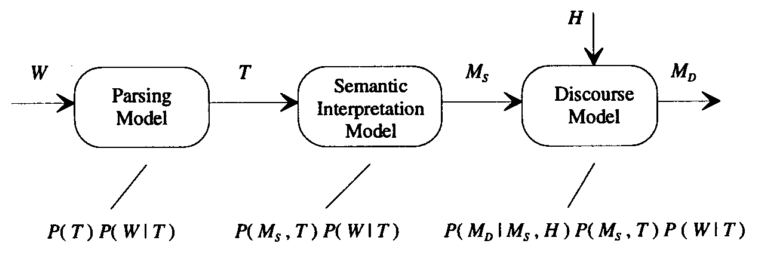
\includegraphics[width=.9\linewidth]{stat_NLI1.png}\\
  \caption{Overview of statistical processing}\label{fig:stat_NLI1}
\end{figure}

This expression corresponds to the computation actually performed by the system which is shown in Figure \ref{fig:stat_NLI1}. The processing proceeds in three stages:
\begin{enumerate}
\item Word string $W$ arrives at the parsing model. The fill space of possible parses $T$ is searched for $n$-best candidates according to the measure $P(T)P(W|T)$. These parses, together with their probability scores, are passed to the semantic interpretation model. The probability $P(T)$ is modeled by state transition probabilities in a recursive transition network, and $P(W|T)$ is modeled by word transition probabilities. Here state transition probabilities have the form $P(state_n | state_{n-1}, state_{up})$, and word transition probabilities have the form $P(word_n | word_{n-1}, tag)$.
\item The constrained space of candidate parses $T$, combined with the full space of possible pre-discourse meanings $M_S$, is searched for $n$-best candidates according to the measure $P(M_s, T)P(W|T)$. These pre-discourse meanings, together with their associated probability scores, are passed to the discourse model. Both pre-discourse and post-discourse meanings in the current system are represented using a simple frame representation (cf. Figure \ref{fig:stat_NLI2}). The problem in this stage is to compute the prior probability of meaning $M_S$ and parse $T$ occurring together. The method of this paper is to embed the instructions for constructing $M_S$ directly into parse $T$. So the probability $P(M_S, T)$ is then simply the prior probability of producing the augmented tree structure.
    \begin{figure}[h]
      \centering
      % Requires \usepackage{graphicx}
      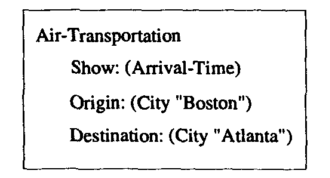
\includegraphics[width=.4\linewidth]{stat_NLI2.png}\\
      \caption{A sample semantic frame}\label{fig:stat_NLI2}
    \end{figure}
\item The constrained space of candidate pre-discourse meanings $M_S$, combined with the full space of possible post-discourse meanings $M_D$, is searched for the single candidate that maximizes $P(M_D | H, M_S)P(M_S, T)P(W|T)$, conditioned on the current history $H$. The discourse history is then updated and the post-discourse meaning is returned. The discourse history $H$ simply consists of the list of all post-discourse frame representations for all previous utterances in the current session. Let $M_P$ denote the last frame in the list. The statistical discourse model maps a 23 element input vector onto a 23 element output vectors. Here $X$ represents the combination of $M_P$ and $M_S$, while $Y$ represents the post-discourse meaning $M_D$. Finally, the probability $P(Y | X)$ is determined by a statistical decision tree model.
\end{enumerate}

In the experimental study, the paper trained and evaluated the system on a common corpus of utterances collected from naive users in the \emph{ATIS} domain. The combined system produced an error rate of 21.6\%, and work on the system was still ongoing.


\subsection{Transparent Combination of Rule-based and Data-driven Approaches in a Speech Understanding Architecture \cite{Rayner2003}}

This paper describes a domain-independent semantic interpretation architecture suitable for spoken dialogue systems, which uses a decision-list method to effect a transparent combination of rule-based and data-driven approaches.

The goal of the paper is to propose an architecture which combines rule-based and data-driven methods as transparently as possible. This will allow the system to shift smoothly from an initial version which is entirely rule-based, to a final version which is largely data-driven.

In this paper, \emph{semantic interpretation} is viewed as a statistical \emph{classification} task. There is a set of semantic atoms, each representing a primitive domain concept, and a semantic representation is defined to be a non-empty set of semantic atoms. For example, the semantic representation of the utterance ``show me the sample syringe'' is $\{show, sample\_syringe\}$. As well as specifying the permitted semantic atoms themselves, it also defines a target model which for each atom specifies the other atoms with which it may legitimately combine. For example, $minutes$ may only combine with $correction$, $set\_alarm$ or a number.

Training data consists of a set of utterances, in either text or speech form, each tagged with its intended semantic representation. The paper defines a set of feature extraction rules, each of which associates an utterance with zero or more features. Statistics are then compiled to estimate the probability $p(a | f)$ of each semantic atom $a$ given each separate feature $f$.

In the decoding process, the system is given an utterance $u$, to which the system assigns a representation $R(u)$ consisting of a set of semantic atoms, together with a target model. The decoding process  proceeds as follows:
\begin{enumerate}
\item Initialise $R(u)$ to the empty set.
\item Use the feature extraction rules and the compiled statistics to find the set of triples $\langle f, a, p \rangle$ where $f$ is a feature associated with $u$, $a$ is a semantic atom, and $p$ is the probability $p(a | f)$.
\item Order the set of triples by the value of $p$, with the largest probabilities first.
\item Remove the highest-ranked triple $\langle f,a,p \rangle$ from $T$. Add $a$ to $R(u)$ if the probability $p$ is greater than some threshold and $a$ is consistent with $R(u)$.
\end{enumerate}

The paper describes an open-source toll called $ALTERF$, which implements the abstract procedure introduced above. It shows how the $ALTERF$ system processes the training data, and decodes the given utterance in running time with further details.

In the experimental study, the paper shows that when all the training data is used, the combined system outperforms the rule-based system by 22.2\% to 27.3\%, and outperforms the N-gram system by 22.2\% to 25.6\%. It shows that the proposed method can get a significant improvement on rules-based technique by adding a trainable component.

\subsection{Incremental LSTM-based Dialog State Tracker \cite{Zilka2015}}

A dialog state tracker estimates the user's goal throughout the dialog by analyzing the \emph{automatic speech recognition (ASR)} outputs for the user's utterance. This paper presents an incremental dialog state tracker based on LSTM networks. It directly uses ASR hypothesis to track the state.

Because of uncertainty in the user input, statistical dialog systems maintain a distribution over all possible states, called the belief state. In this paper, a dialog state at time $t$ is defined as a vector $s_t \in C_1 \times ... \times C_k$ of $k$ dialog state components (sometimes also called slots). Each component $c_i \in C_i = \{ v_1, ..., v_{n_i} \}$ takes one of $n_i$ values. The goal of the dialog state tracker is to give the probability distribution over one of the independent components $p(c_i | w_1, ..., w_t)$.

\begin{figure}[h]
  \centering
  % Requires \usepackage{graphicx}
  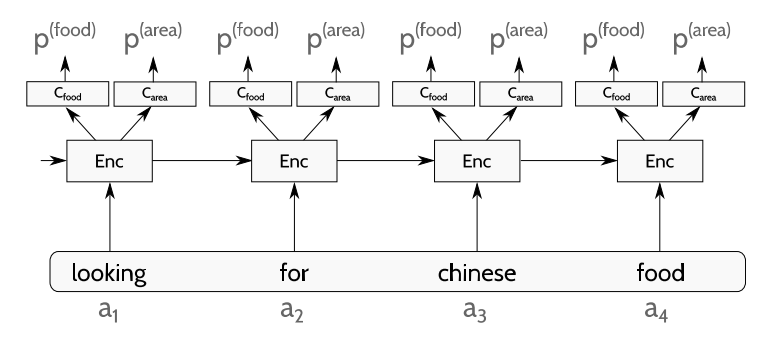
\includegraphics[width=.7\linewidth]{11_28_dstc_ilstm.png}\\
  \caption{A demonstration of the proposed model}\label{fig:dstc_ilstm}
\end{figure}

The main idea of this paper is to use LSTM to encode the information from the input word sequence into a fixed-length vector representation. Given this representation, a classifier returns a probability distribution over the value of the dialog state. An example of the model applied to a particular input sentence is at Figure \ref{fig:dstc_ilstm}.

Formally, the input neural network maps the word $a$ and its ASR confidence score $r$ to a joint representation $u$: $u = NN(a, r)$. The representation $u$ is used by the LSTM encoder along with the previous hidden state $q_{t-1} = (c_{t-1}, h_{t-1}$ to create a new hidden state $q_t$: $q_t = Enc(u, q_{t-1})$. The classifier, represented by a single softmax layer, then maps the hidden state to a probability distribution over all possible values: $p_t = C(h_t)$.

The training criterion is a cross-entropy loss for a dialog example, which is annotated by true labels at some points in time:
$$l(\theta) = - \sum_{t \in Y} \log LecTrack(a_1, r_1, ..., a_n, r_n)_{y_t}^t,$$
where $y_i$ denotes a label for the dialog state at time $i$, and $Y$ is a set of times where the label $y_i$ exists.

In the experimental study, the paper shows that the propose model yields performance to the state-of-the-art system. For example in the requested component, the proposed method achieves 0.98 accuracy and 0.04 L2 score, which is identical to the result of the previous best system.

\section{Dialogue Manager}

The \emph{DM (dialogue manager)} component deals with (1) \emph{state tracking}, which refers to representing information from the past as dialogue states; (2) \emph{action selection}, which refers to mapping from dialogue states to system actions.

Dialogue states can be hand-coded and human-interpretable. They usually consist of \emph{user goals}, like the preferred price range of a restaurant, and \emph{dialogue history}, like whether the address of a restaurant has been asked for (see Table \ref{Goal-Oriented Dialogue System Example} for an example). Methods, like recurrent neural networks \cite{Henderson2014Word}, can be used to learn from data how to update the state. Action selection may be learned via reinforcement learning as in \emph{Markov decision process (MDP)} \cite{Levin2000A} and \emph{partially observable Markov decision process (POMDP)} \cite{Young2013Pomdp, Gasic2011}. MDP learns to map dialogue states to actions and does not model the uncertainty about states. To tackle the problem, POMDP maintains a distribution over dialogue, i.e. \emph{belief state}, and based on the distribution actions are chosen.

Hand-crafting dialogue states can be quite labor intensive. Williams et. al propose to automatically infer state representation using neural networks \cite{Williams2016End}. Similarly, Bordes et al. show that an end-to-end trainable system can reach promising performance without hand-crafted features for dialogue states.

\subsection{End-to-end LSTM-based dialog control optimized with supervised and reinforcement learning \cite{Williams2016End}}

The paper presents a model for end-to-end training of goal-oriented dialogue systems, which breaks the operational loop of a dialogue system down into 13 steps (Figure \ref{fig:Williams2016End01}). The model combines recurrent neural networks and domain-specific software that expresses business rules and provides API access in the domain. The recurrent neural networks automatically infer dialogue state representation, and thus hand-coded state features are not needed.

\begin{figure}[htbp]
  \centering
  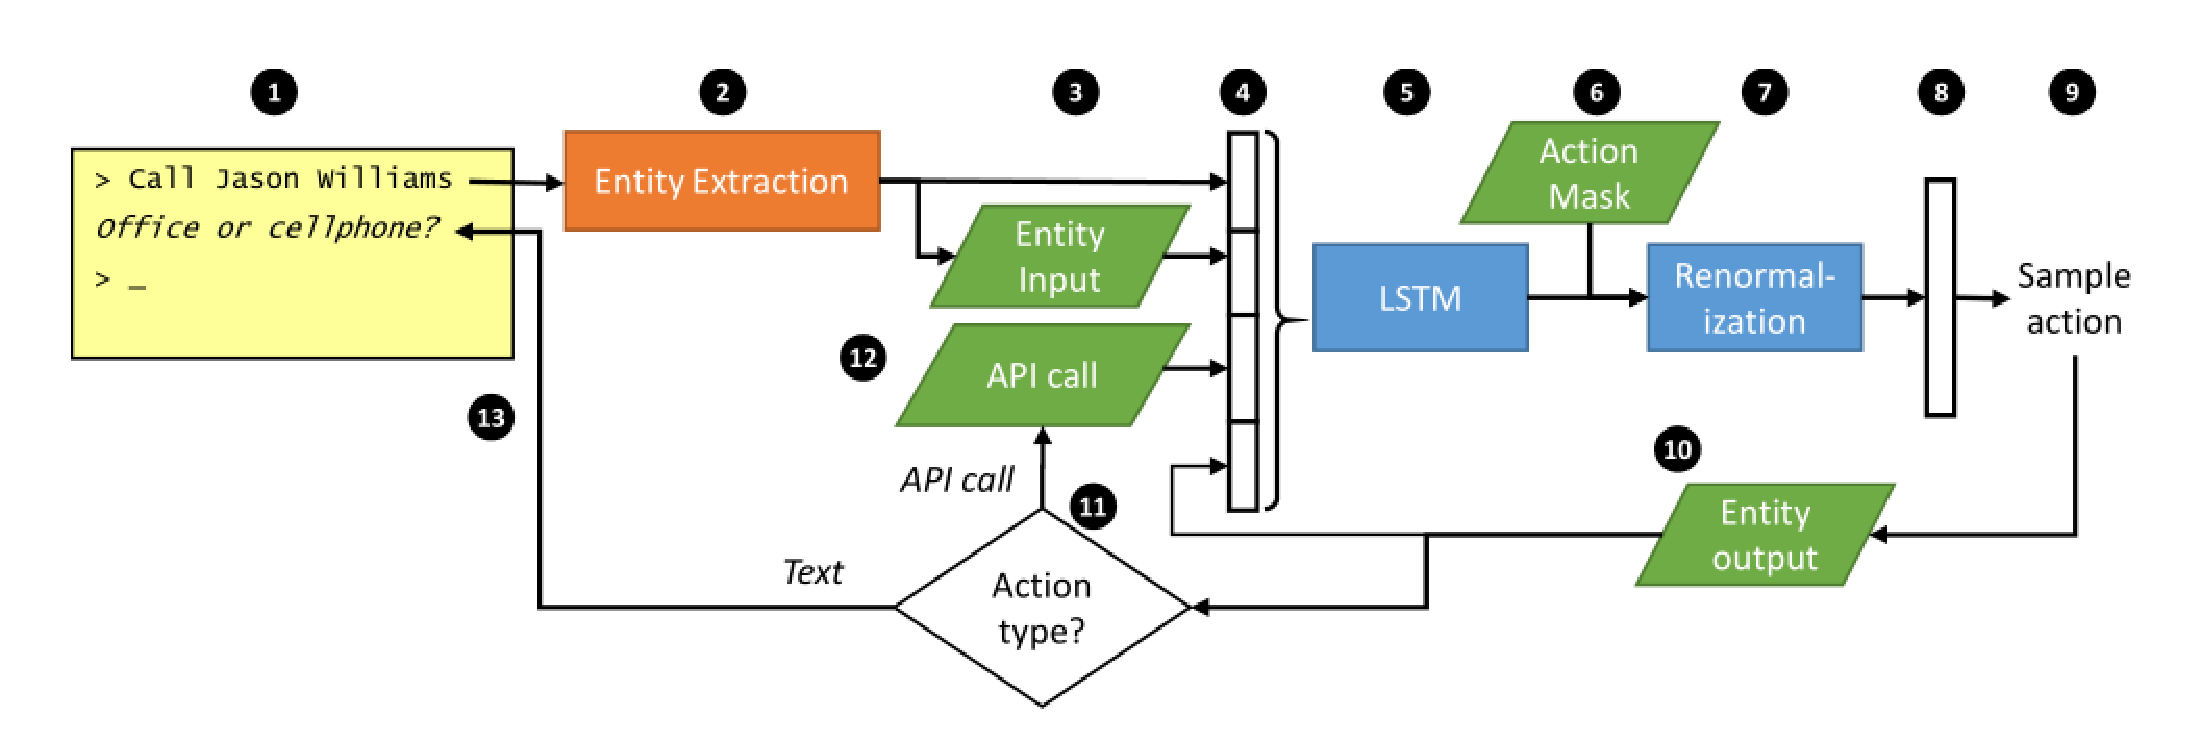
\includegraphics[width=\linewidth]{Williams2016End01}\\
  \caption{Operational loop of a dialogue system}\label{fig:Williams2016End01}
\end{figure}

The operational cycle has 13 steps: (1) The system receives user input; (2) The entities mentioned in user input are identified; (3) The extracted entities are resolved into ground entities corresponding to one or more rows in a database; (4) A feature vector is constructed from four sources; (5) LSTM takes the feature vector, update its hidden states, and outputs a distribution over all template actions; (6) Domain-specific software provides an action mask indicating actions that are not allowed at the current time; (7, 8) The task mask is combined with the distribution in step five into a new distribution; (9) An action is chosen from the new distribution; (10) The selected template action is instantiated with the entities in step three; (11, 12, 13) Depending on the action type, the system either invokes the corresponding API call or render the response text to users.

\subsection{Learning End-to-End Goal-Oriented Dialog \cite{Bordes2016Learning}}

The main contributions of the paper are: (1) propose to evaluate end-to-end dialogue systems using goal-oriented tasks, and design five tasks in the application of restaurant reservation; (2) apply Memory Networks to train an end-to-end dialogue system, and show that per-response performance is encouraging.

The five tasks are (1) issue API calls. The system should ask questions, gather information about the preferred cuisine type, location, price range, and party size of restaurants, and generate the correct API call; (2) update API calls. When user preferences change, the system should update the API call; (3) display options. The system should propose the restaurants, which match user preferences, until users accept; (4) provide extra information. When users ask for the phone numbers and address of a restaurant, the system should answer correctly based on the facts; (5) conduct full dialogues (see Figure \ref{fig:Bordes2016Learning01} for examples of the five tasks). Natural language patterns and knowledge base entities are combined to generate simulated dialogues consisting of user and system utterances.

\begin{figure}[htbp]
  \centering
  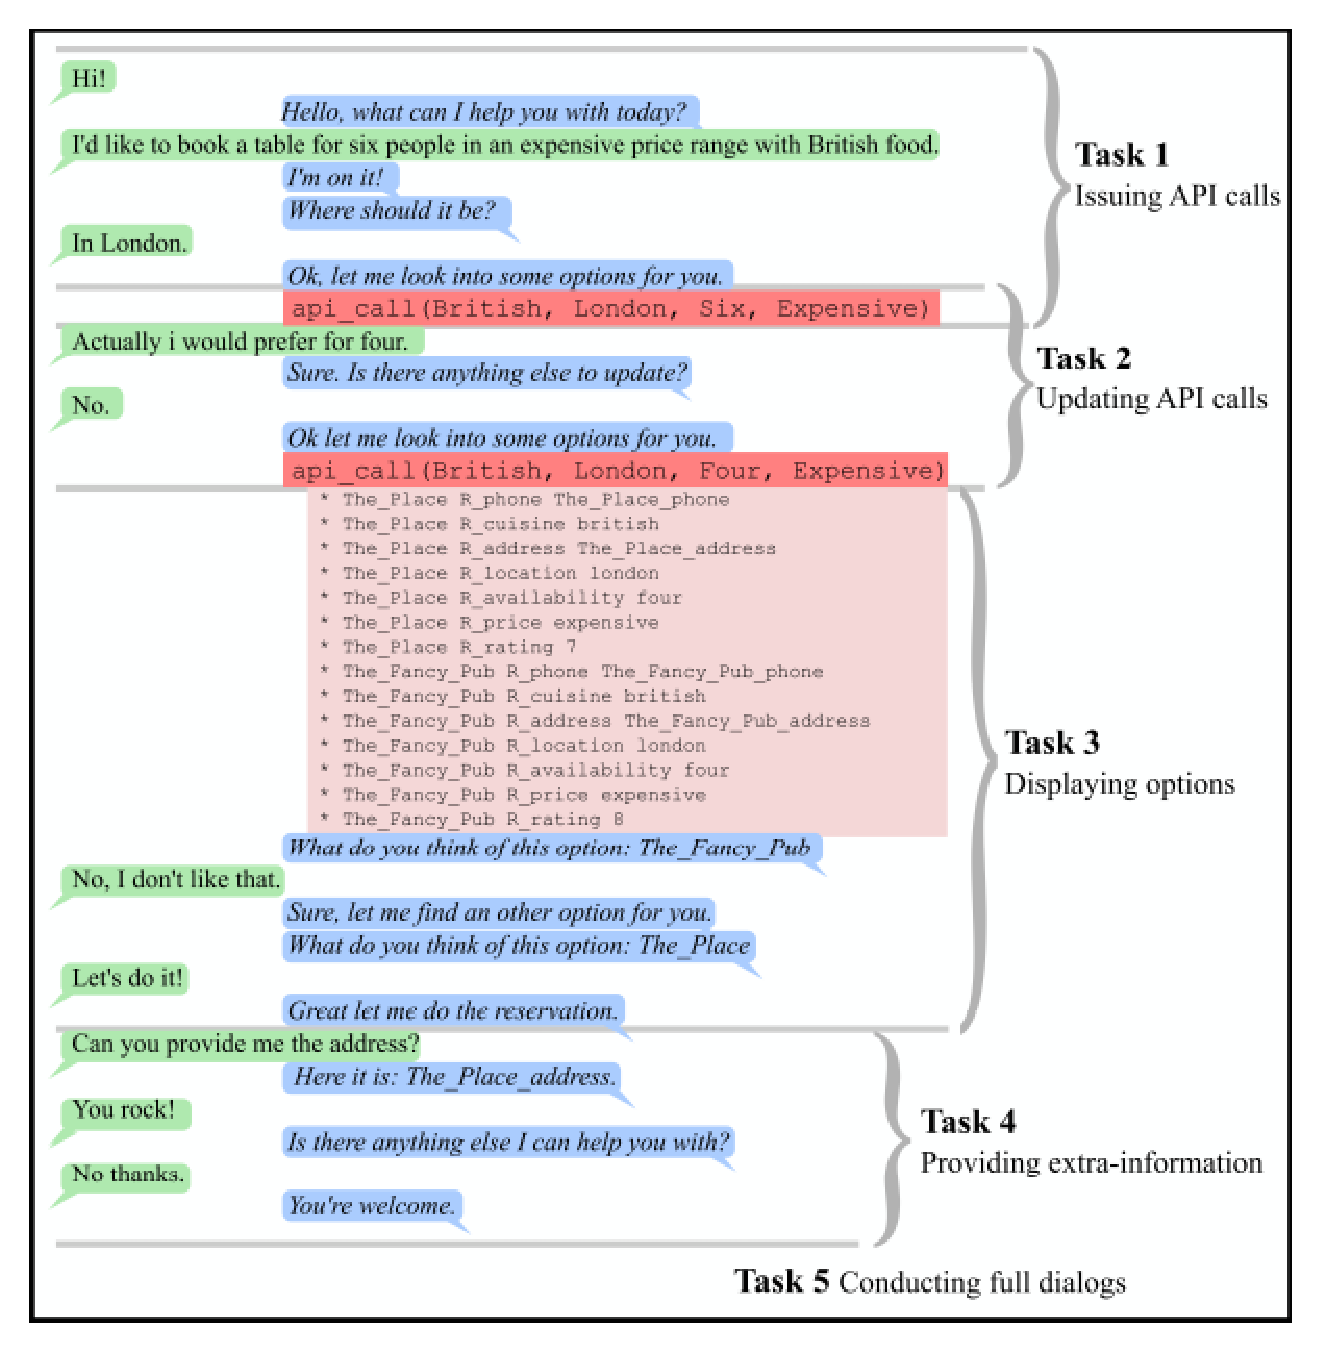
\includegraphics[width=.8\linewidth]{Bordes2016Learning01}\\
  \caption{Examples of the five tasks}\label{fig:Bordes2016Learning01}
\end{figure}

The paper uses a retrieval-based method, i.e. selecting the best candidate response from a large set of all possible system utterances and API calls. The paper applies Memory Networks that consist of three component (1) store conversation in memory; (2) read pertinent information from the memory; (3) use the information to output the best candidate response.

\subsection{Word-based dialog state tracking with recurrent neural networks \cite{Henderson2014Word}}

The task is to converts user inputs into dialogue states (see Table \ref{Goal-Oriented Dialogue System Example} for an example of dialogue state). The dialogue state is a probability distribution over handcrafted goals, methods, and requested slots. The paper uses a RNN to compute the distribution over goal values for each goal, a RNN to compute the distribution over methods, and a RNN to compute the distribution over requested slots. During training, gradient clipping is used to avoid exploding gradients \cite{Pascanu2012Understanding}.

\begin{table}[!hbp]
\begin{tabular}{|r|rl|}
\hline
\textbf{System Output} & \multicolumn{2}{l|}{You can ask for restaurants by area, price range or food type.} \\
\hline
\textbf{User Input} & \multicolumn{2}{l|}{Expensive restaurant in the south part of town.} \\
\hline
\emph{Dialogue State} & goals
& 0.7 pricerange=expensive area=south \\
&& 0.2 pricerange=expensive area=north \\
& methods & 0.9 method=byconstraints \\
&& 0.1 method=byalternatives \\
& requested slots & 0.0 address \\
&& 0.0 phone \\
\hline
\emph{System Act} & \multicolumn{2}{l|}{request(food)} \\
\hline
\textbf{System Output} & \multicolumn{2}{l|}{What kind of food would you like?} \\
\hline
\end{tabular}
\caption{Goal-Driven Dialogue System} \label{Goal-Oriented Dialogue System Example}
\end{table}

\subsection{On-line policy optimisation of Bayesian spoken dialogue systems via human interaction \cite{Gasic2011}.}

The task is to learn system policy, which determines system acts based on dialouge states (see Table \ref{Goal-Oriented Dialogue System Example} for an example). The paper applies GP-Sarsa to automatic policy learning, which is an online RL algorithms based on Gaussian process \cite{Engel2014Reinforcement}. The GP-Sarsa optimization adopts a more robust filtered reward function \cite{Gašić2011Online}.

\subsection{A stochastic model of human-machine interaction for learning dialog strategies \cite{Levin2000A}}

This paper proposes a quantitative model for dialog systems that can be used for learning the dialog strategy. After formalising the dialog design as a \emph{Markov decision process (MDP)}, the reinforcement learning algorithm is used to find the optimal strategy. This approach is evaluated in an \emph{air travel information system (ATIS)} task.

The key idea of this paper is to formalise the dialog design as an optimization problem with an objective function reflecting different dialog dimensions for a given application. With some assumptions about the state transition probabilities and cost assignment, a dialog system can be mapped to a MDP, which has a variety of data driven algorithms for finding the optimal strategy.

The first step is to state the problem of dialog design as optimization of an objective $C$:
$$C = \sum W_i \langle C_i \rangle,$$
where the terms $\langle C_i \rangle$ are the expected costs for different dialog dimensions. The paper illustrates the concepts with a toy example of ``Day-and-Month Dialog'', where the goal is to get the correct day and month values from the user. In the case, the objective $C$ has three components: the first part denotes the \emph{expected duration} of the dialog; the second part denotes the expected number of error; the last part corresponds to the expected distance from achieving the application goal. With this concept, the goal of a dialog system is to minimize the cost function.

\begin{figure}[htbp]
  \centering
  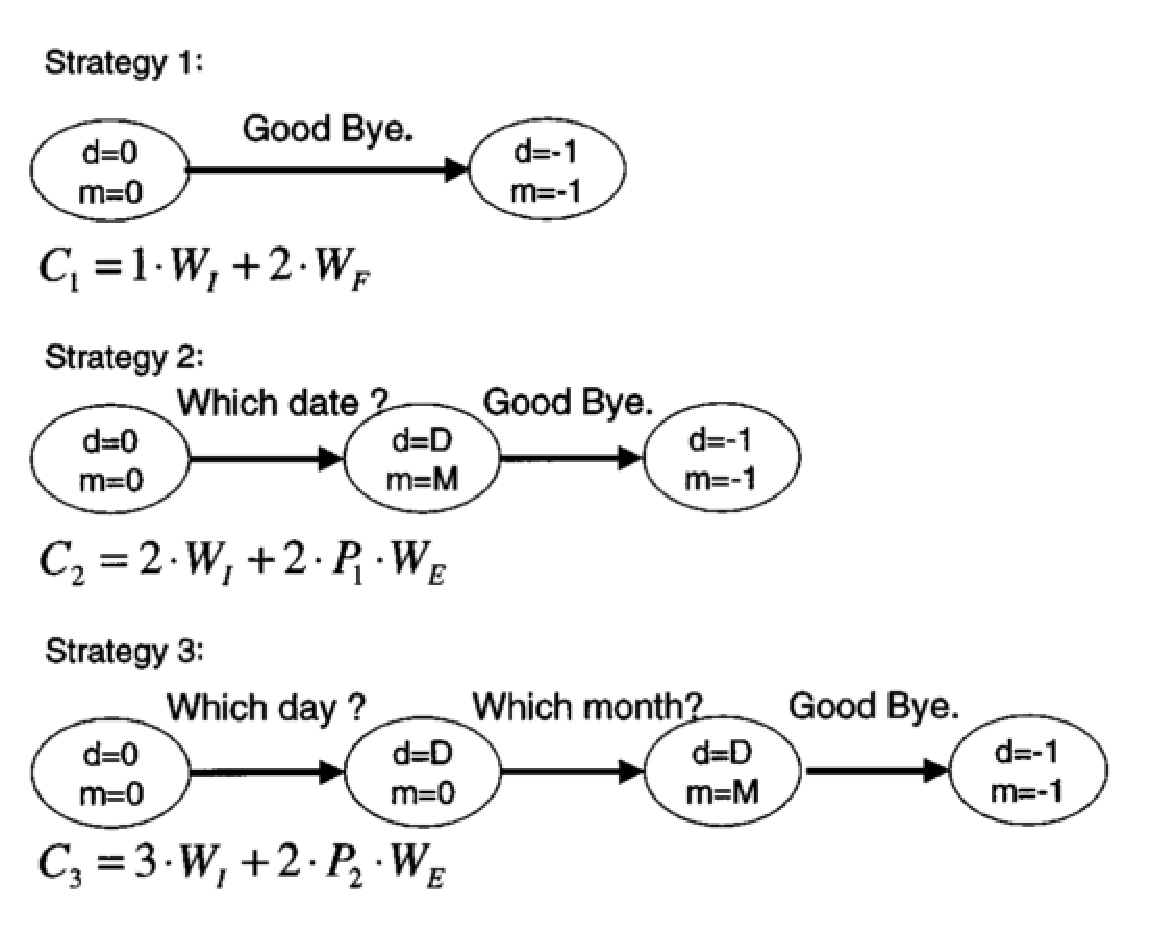
\includegraphics[width=.6\linewidth]{10_17_dialog_MDP1}\\
  \caption{Three possible strategies for the day-month dialog system}\label{fig:dialog_MDP1}
\end{figure}

The next step is to formalize a dialog system as a sequential decision process in terms of its action set, state space, and strategies: 1) The action set of the dialog system includes all possible actions it can perform, such as interactions with the user (e.g., asking the user for input, providing some output, etc.). In the toy example, there are four actions, such as asking for the day $A_d$, asking the month $A_m$, asking the date (day and month) $A_{dm}$, and a final action $A_f$; 2) The state $s$ includes the values of all relevant variables that determine the next action. In the example each state has two integer variables, $d \in \{0, ..., 31\}$ and $m \in \{0, ..., 12\}$, corresponding to the day and month respectively. 3) A dialog strategy maps each state to an action. For example, Figure \ref{fig:dialog_MDP1} shows three possible strategies for the example system.

With some assumptions about the transition probabilities between states, and the cost assignment, the sequential decision process can be formalise as a MDP. Then the optimal strategy can be obtained by a variety of reinforcement learning algorithms.

However, in reinforcement learning, the optimal strategy is learned not from a static corpus but through interaction, because the strategy itself determines the distribution of states in the corpus. To overcome this problem, the paper proposes the use of a \emph{simulated user}. The simulated user is a stochastic generative model that produces speech acts as a response to a dialog action. The simulated user does not deal with the language understanding component - it communicates with the dialog system through semantic representations. The parameters of the simulated user can be estimated from an annotated dialog corpus.

\begin{figure}[htbp]
  \centering
  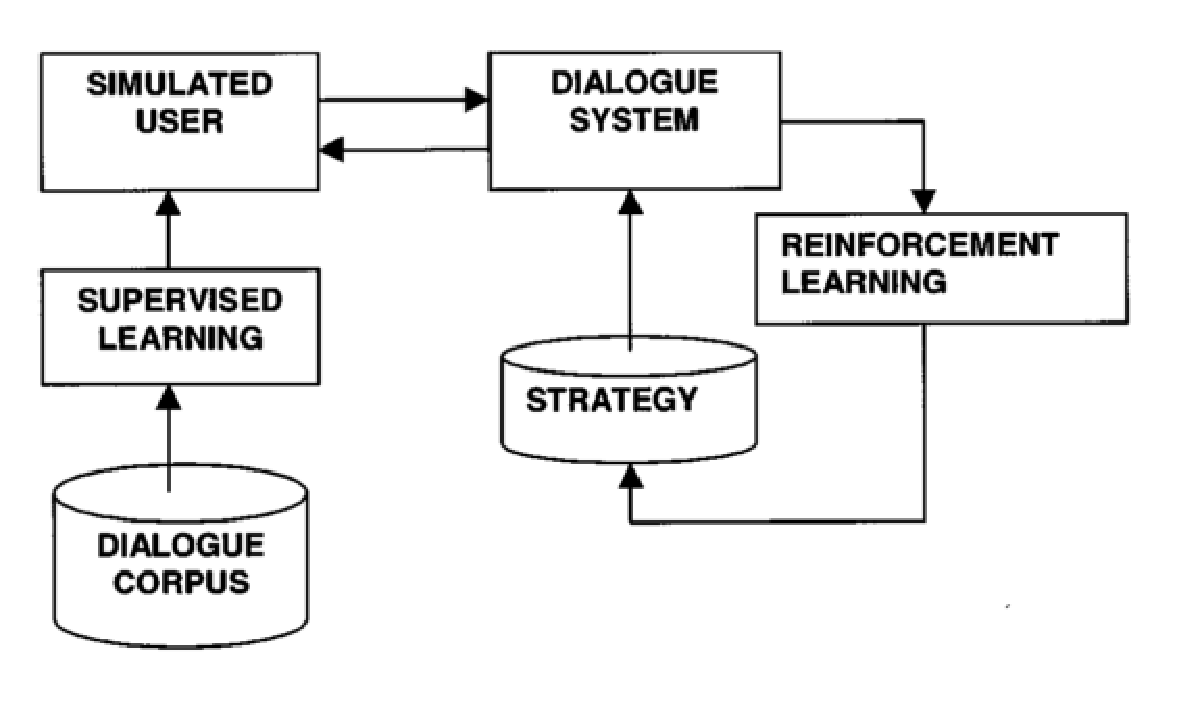
\includegraphics[width=.6\linewidth]{10_17_dialog_MDP2}\\
  \caption{Procedural description of the learning paradigm}\label{fig:dialog_MDP2}
\end{figure}

Once a simulated user is available, it can be used in a generative mode for interacting with the dialog system while the reinforcement learning algorithm is estimating the optimal strategy. Then when a reasonable estimate of the optimal strategy is obtained, the system can be used with real users and the learning process can continue. Figure \ref{fig:dialog_MDP2} summarizes the suggested learning paradigm.

\begin{figure}[htbp]
  \centering
  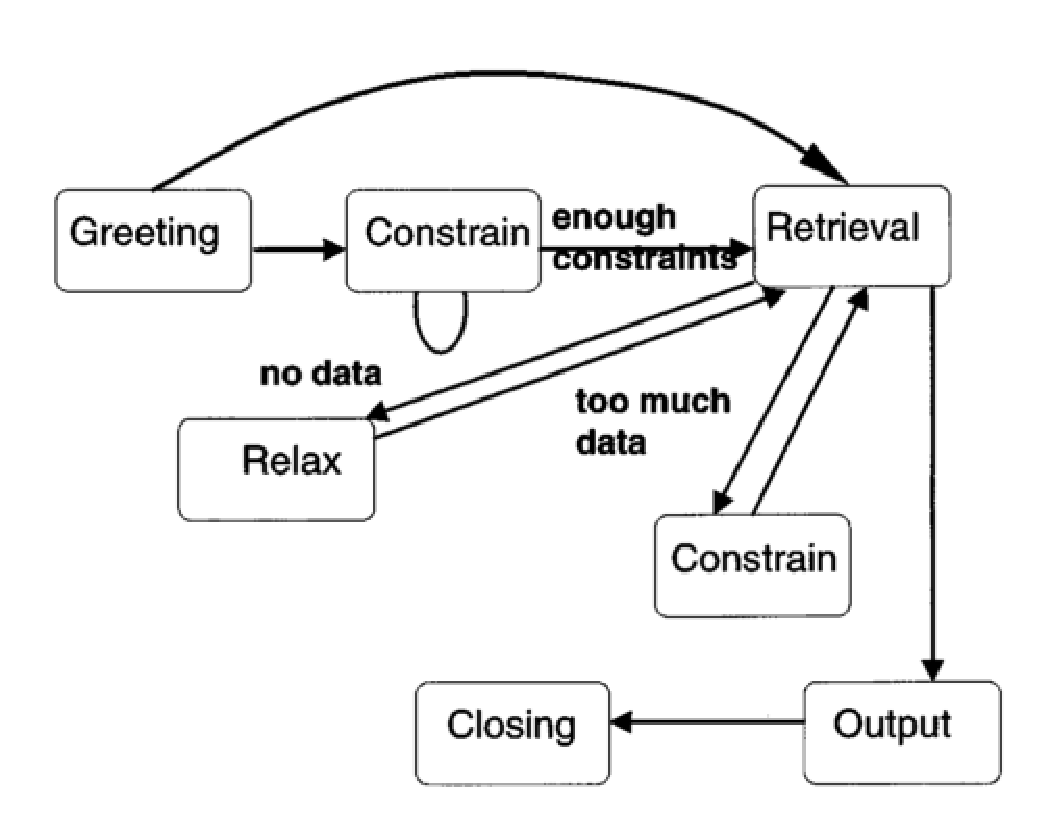
\includegraphics[width=.5\linewidth]{10_17_dialog_MDP3}\\
  \caption{Schematic representation of the optimal strategy for ATIS}\label{fig:dialog_MDP3}
\end{figure}

In the experimental study, the paper shows that a nontrivial strategy can be automatically learned given the simple objective function. For example, Figure \ref{fig:dialog_MDP3} shows the learned strategy of the ATIS task.

Remark: I have also considered formalising the dialog manager as a MDP, and realised one obvious difficulty is that there is not an interactive environment to train the system. This paper introduces simulated users to overcome this difficulty. Another good idea is to abstract the dialog process, such as using semantic representations without considering the ASR or NLU component. I think this paper shows a very promising approach for building our chatbot.

\subsection{POMDP-based Statistical Spoken Dialogue Systems: a Review \cite{Young2013Pomdp}}

By including an explicit Bayesian model of uncertainty and by optimising the policy via a reward-driven process, \emph{partially observable Markov decision processes (POMDPs)} provide a data-driven framework that reduces the cost of hand-crafting dialog managers and provides robustness against the errors created by speech recognisers operating in noisy environments. This paper provides an overview of the current state of the art in the development of \emph{POMDP-based spoken dialog systems (SDS)}.

\begin{figure}[htbp]
  \centering
  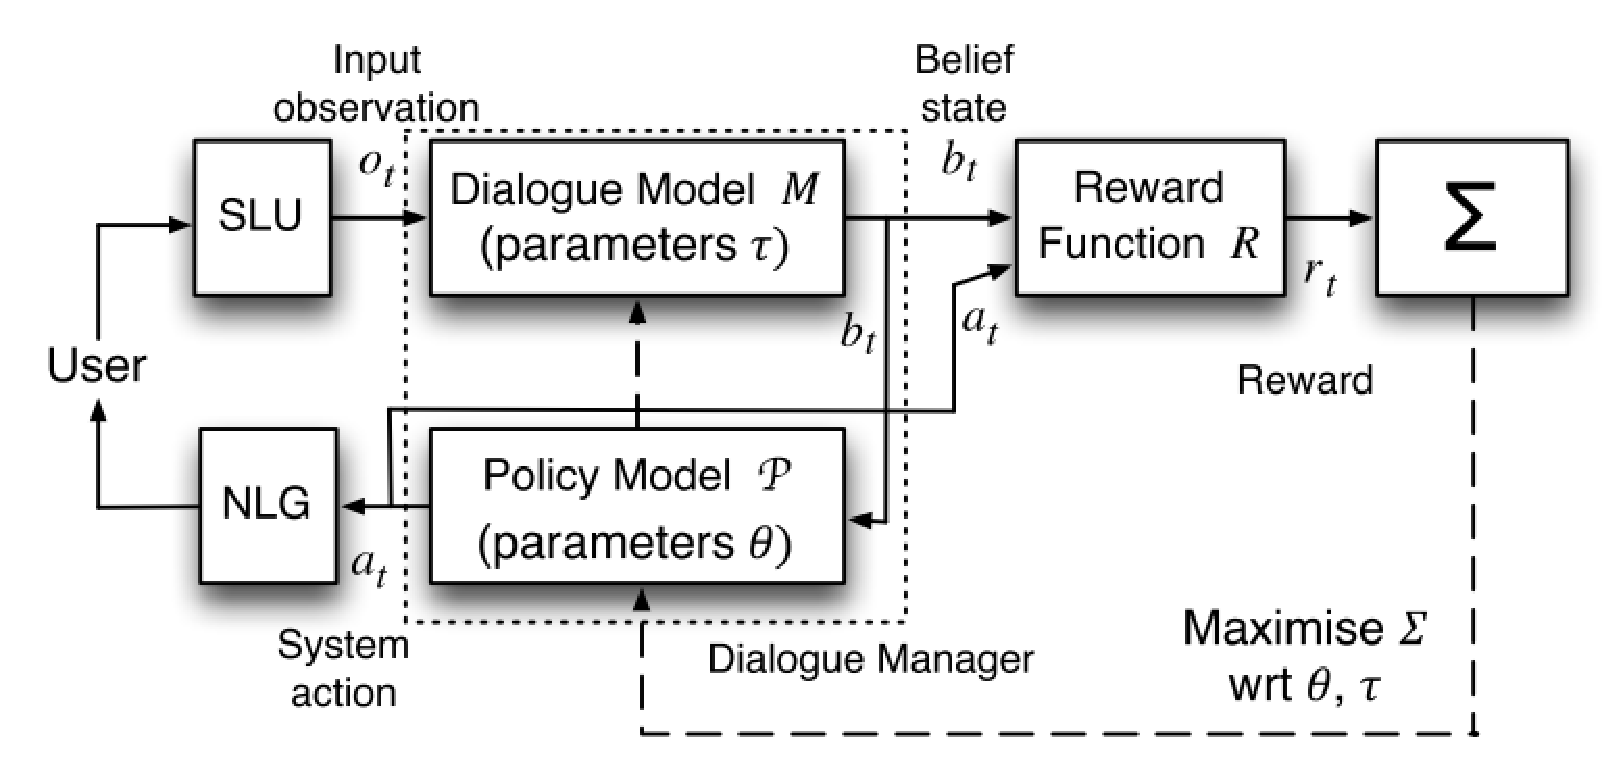
\includegraphics[width=.7\linewidth]{10_17_POMDP1}\\
  \caption{Components of a POMDP-based spoken dialog system}\label{fig:POMDP1}
\end{figure}

%The principal elements of a conventional Spoken Dialog System (SDS) are shown in Figure \ref.
The POMDP approach assumes that dialog evolves as a Markov process, i.e., starting in some initial state, each subsequent state is modelled by a transition probability $p(s_t | s_{t-1}, a_{t-1})$. The state $s_t$ is not directly observable. At each turn, the system regards the output of the SLU as a noisy observation $o_t$ of the user input with probability $p(o_t | s_t)$. The transition and observation probability functions are represented by the dialog model. The decision as to which action to take is represented by the policy. The components of a POMDP-based system are presented in Figure \ref{fig:POMDP1}.

\begin{figure}[htbp]
  \centering
  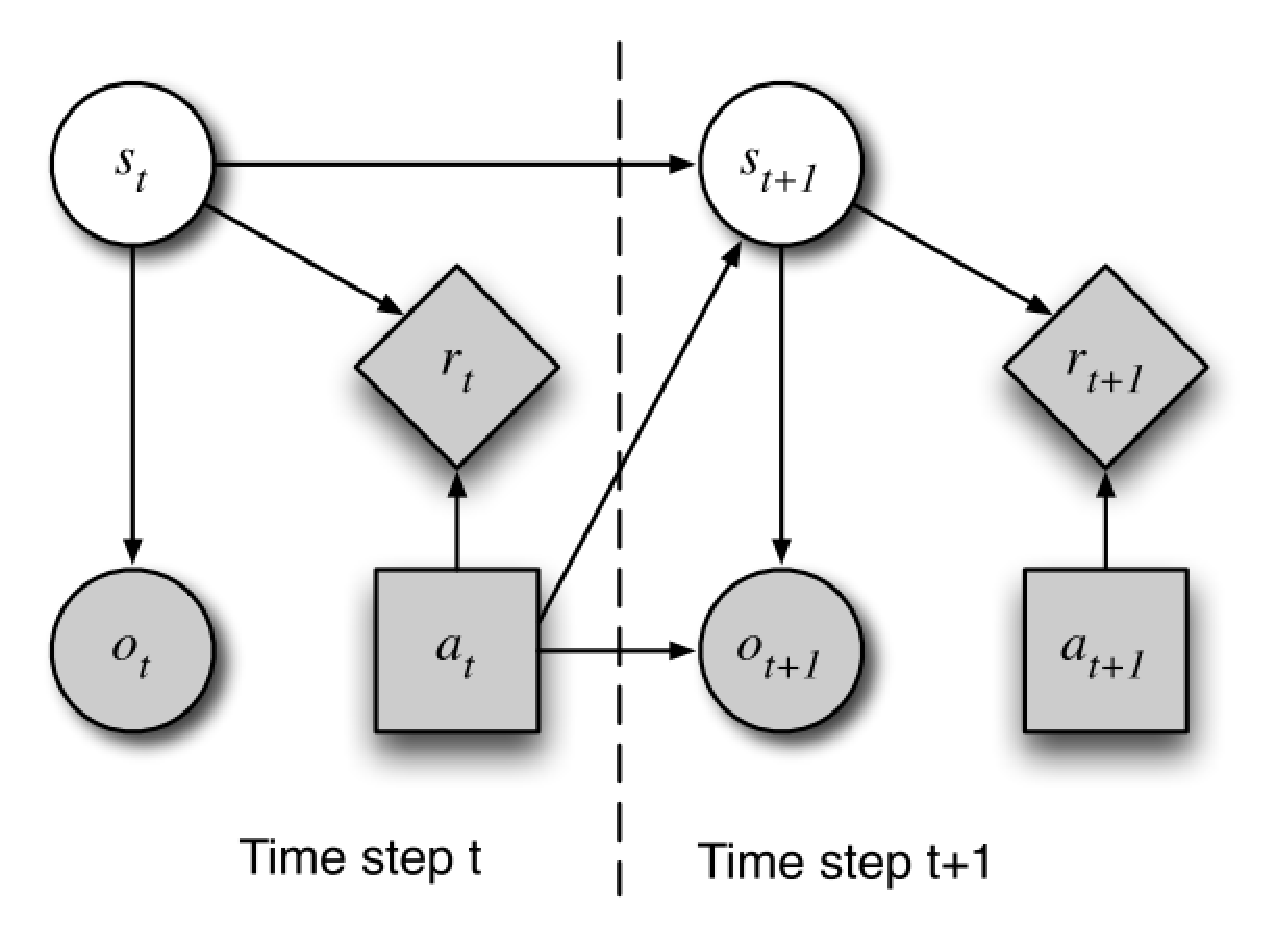
\includegraphics[width=.5\linewidth]{10_17_POMDP2}\\
  \caption{An influence diagram of a POMDP}\label{fig:POMDP2}
\end{figure}

The paper first introduces some preliminary knowledge about the POMDP method. In a POMDP system in each step the world is in some unobserved state $s_t$. Since $s_t$ is not known exactly, a distribution over possible states called a belief state $b_t$ is maintained, where $b_t(s_t)$ indicates the probability of being in a particular state $s_t$. Based on $b_t$, the machine selects an action $a_t$, receives a reward $r_t$, and transitions to (unobserved) state $s_{t+1}$. The machine then receives an observation $o_{t+1}$. This process is represented as an influence diagram in Figure \ref{fig:POMDP2}.

Given an existing belief state $b_t$, the last system action $a_t$, and a new observation $o_{t+1}$, the new updated belief state is given by:
$$b_{t+1}(s_{t+1}) = \eta P(o_{t+1} | s_{t+1}, a_t) \sum_{s_t} P(s_{t+1} | s_t, a_t)  b_t(s_t),$$
where $\eta$ is a normalization constant. The system action is determined by a policy $\pi$. The discounted sum of rewards expected by starting in $b_t$ and following policy $\pi$ is given by the value function $V^\pi(b_t)$. In POMDP, finding an optimal policy is called solving or optimizing the POMDP. However, standard POMDP methods do not scale to the complexity needed to represent a real-world dialog system. So the next sections of this paper introduce some domain-specific methods for applying POMDP in the SDS task.

The first step is to review some possible approaches to represent the dialog model. In a goal-oriented SDS, the state should encode three distinct types of information: the user's goal $g_t$, the intent of the most recent user utterance $u_t$, and the dialog history $h_t$. The resulting influence diagram is shown in Figure \ref{fig:POMDP2}, in which some reasonable independence assumptions have been introduced. Factoring the state in this way can significantly reduce the POMDP model complexity. However, it is still too complex to support tractable real-world systems, so further approximation is necessary. The paper introduces two main approaches: the N-best approach, and the factored Bayesian Network approach.

In N-best approaches, the belief state is approximated by a list of the most likely states with their probabilities. It can also be viewed as running N conventional dialog systems in parallel, such that each parallel thread tracks a different interpretation of what the user said.

\begin{figure}[htbp]
  \centering
  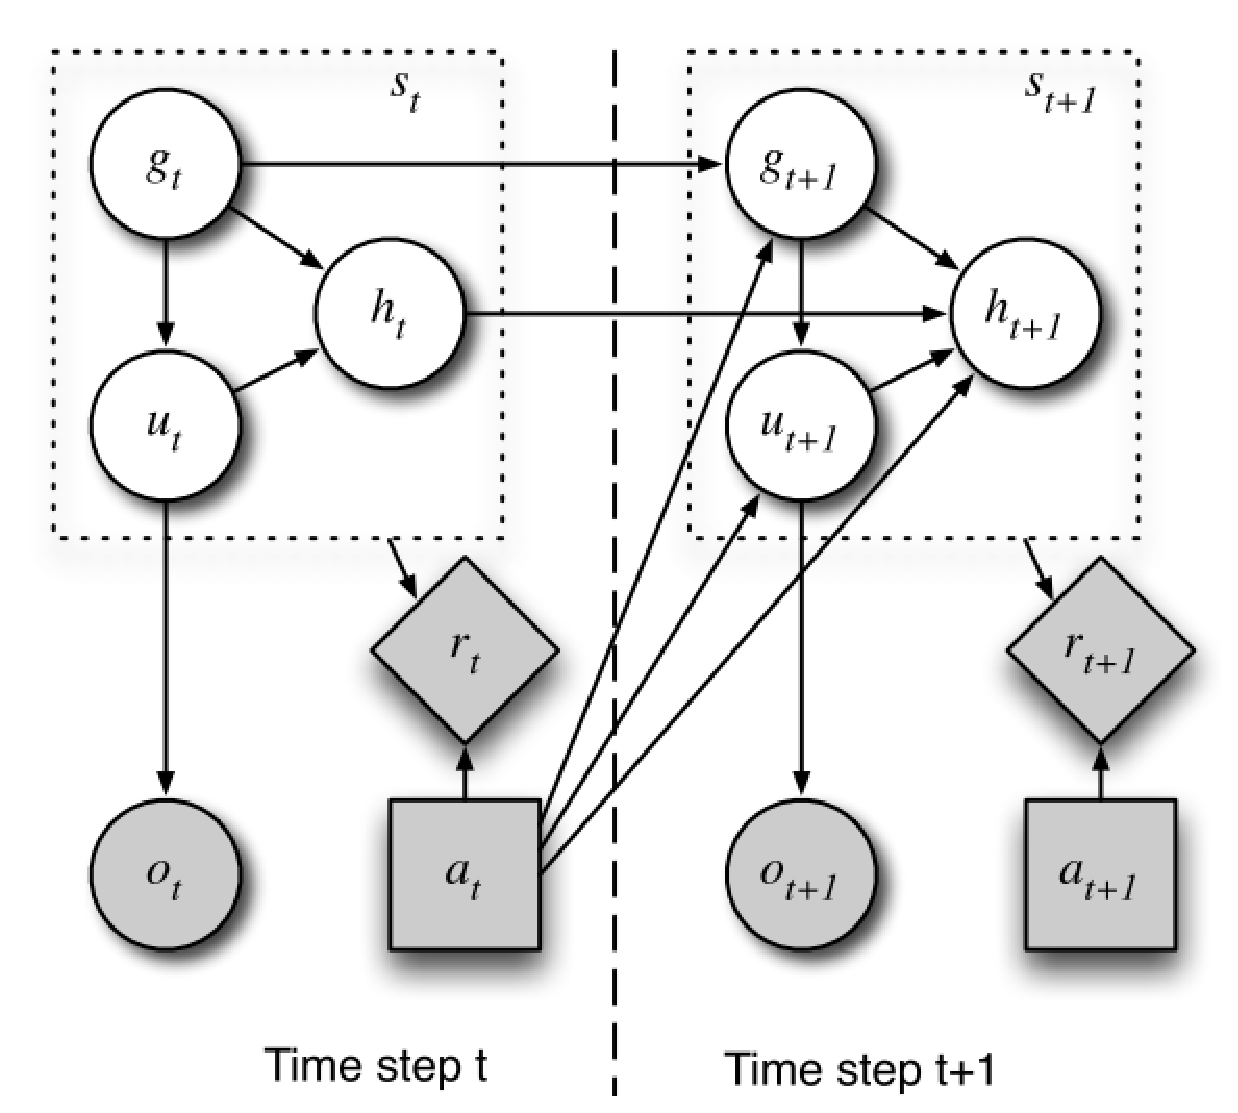
\includegraphics[width=.5\linewidth]{10_17_POMDP3}\\
  \caption{An influence diagram of a factored state POMDP}\label{fig:POMDP3}
\end{figure}

The second approach is to factor the user goal into concepts that can be spoken about by the system. This is illustrated in Figure \ref{fig:POMDP3}, which shows an example from a tourist information system, in which entities have a type, the kind of food served and an area.

The next big challenge of a POMDP-based system is the representation and estimation of the policy model. The paper presents five different methods of policy optimisation: planning under uncertainty, value iteration, Monte-Carlo optimisation, least-squares policy iteration, and natural actor-critic. These methods have been selected because all have been applied to end-to-end working dialog systems.

Another problem is also mentioned in the previous paper summaries of the MDP-based approaches: learning directly from corpora is problematic, because an interactive environment is necessary. One solution is to build a model of the user that can interact directly with a dialog system, and which can itself be trained on corpora. In a real system the dialog manager only has access to a noisy observation, so an error model is needed as well as a user model.

The following three sections presents some more advanced techniques for dialogue model parameter optimisation, fast training, user adaption, and discusses some real-world systems and applications. Finally, the paper discusses the current evaluation methods of SDS. Evaluation of SDS typically falls into one of 3 testing regimes: testing with some form of simulated user, testing with paid subjects, and testing within a live deployed system.

Remark: I am not very familiar with the POMDP approach, so some of the technical details mentioned in the paper are still not very clear to me. Intuitively, POMDP should have better performance than MDP (but also harder to train). I think it is also possible to combine it with the deep learning techniques, such as representing the transition probabilities with a neural network approximately.

\section{Natural Language Generation}

The generation component of a conversational agent chooses the concepts to express to the user, plans out how to express these concepts in words, and assigns any necessary prosody to the words \cite{Jurafsky2006}. In other words, the NLG component generates surface texts based on abstract system actions \cite{Wen2015Stochastic}. Language models can be used to rerank the generated texts \cite{Martens2011, Bengio2003A}.

One of the most recent important technique in the field of natural langue processing is the word-embedding technique, which learns a distributed representation of each word. In this section, we begin with introducing one of the classic paper of the word-embedding techniques \cite{Bengio2003A}. The next two papers then shows how the new emerged deep learning methods, particularly the recurrent neural networks, are applied in the NLG component.

\subsection{A Neural Probabilistic Language Model \cite{Bengio2003A}}

This paper proposes a neural network architecture to learn a probabilistic language model. The method can simultaneously learn a distributed representation for each word and the probability function for word sequences.

A goal of statistical language modeling is to learn the joint probability function of sequences of words in a language. It can be represented by the conditional probability of the next word given all the previous ones:
$$P(w_1^T) = \prod_{i=1}^T P(w_t | w_1^{t-1}).$$
Here $w_t$ is  the $t$-th word, and $w_i^j = (w_i, w_{i+1},... , w_j)$ is the subsequence from the $i$-th to the $j$-th word.

One of the motivations of this paper is that traditional $n$-gram models do not take into account of the similarity between words. For example, having seen the sentence ``The cat is walking in the bedroom'' in the training corpus, a model should assign high probability to the sentence ``A dog was running in a room'', because ``the'' and ``a'', ``dog'' and ``cat'' are similar to each other.

The basic idea of the proposed approach can be summarized as follows: 1) Associate with each word a distributed word feature vector (a real-valued vector in $\mathbb{R}^m$); 2) Express the joint probability function of word sequences in terms of the feature vectors; 3) Learn simultaneously the word feature vectors and the probability function.

Specifically, the objective of the neural network is to learn a good model $f(w_t, ..., w_{t-n+1}) = P(w_t | w_1^{t-1})$. The function $f(w_t, ..., w_{t-n+1})$ is decomposed in two parts:

\begin{enumerate}
\item A mapping $C$ from any element $i$ from the vocabulary $V$ to a real vector $C(i) \in \mathbb{R}^m$. It represents the distributed feature vectors associated with each word.
\item The probability function over words, which is denoted by $g$. The input of $g$ is a sequence of feature vectors of words in context ($C(w_{t-n+1}),..., C(w_{t-1})$), and the output is a vector whose $i$-th element estimates the probability of next word being $i$ ($P(w_t = i | w_1^{t-1})$).
\end{enumerate}

\begin{figure}[htbp]
  \centering
  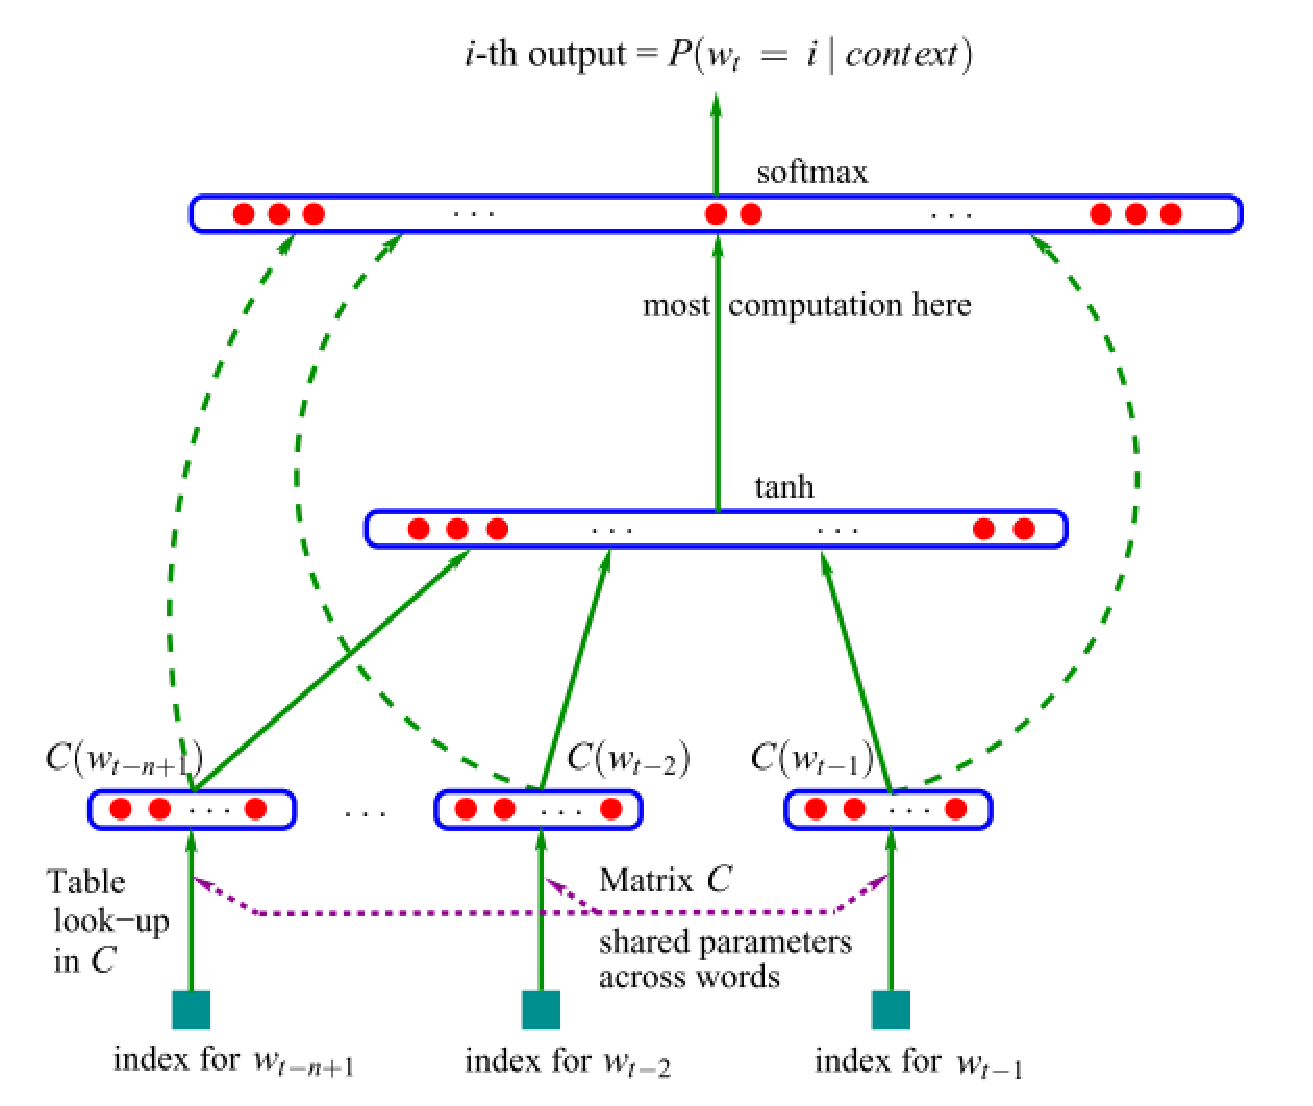
\includegraphics[width=.8\linewidth]{8_15_DL}\\
  \caption{An overview of the network architecture}\label{fig:DL}
\end{figure}

Figure \ref{fig:DL} shows the proposed neural architecture. The objective  function $f$ is a composition of $C$ and $g$, with $C$ being shared across all the words in the context. The function $g$ can be implemented by a feed-forward or recurrent neural network. This paper uses the ordinary hyperbolic tangent hidden layer with a softmax output layer.

The paper also explores parallelization on two types of platforms: shared-memory processor machines and Linux clusters with a fast network. In the case of a shared-memory processor, each processor works on a different subset of the data. Each processor computes the gradient for its examples, and performs stochastic gradient updates on the parameters of the model, which are simply stored in a shared-memory area. If the parallel computer is a network of CPUs, the paper chooses to parallelize across the parameters of the output units. The CPUs need to communicate the normalization factor of the output softmax, and the gradients on the hidden layer with the word feature layer. All the CPUs will duplicate the computations that precede the output units. After this step, each processor works on its local data as before.

In this experimental section, the paper measures the perplexity of the proposed model, and compares the results with several previous work. It is reported that the proposed method outperforms the most competitive alternative approach by up to 24\% in perplexity.


\subsection{Stochastic language generation in dialogue using recurrent neural networks with convolutional sentence reranking \cite{Wen2015Stochastic}}

The task is to maps system acts into surface texts. The paper uses RNN LM to generate responses by sampling words from the predicted distribution conditioned on dialogue acts. After generating response candidates, CNN and RNN are used together to score and rerank the candidates.

\subsection{Generating Text with Recurrent Neural Networks \cite{Martens2011}}

This paper proposes a new variant of \emph{Recurrent Neural Network (RNN)} called \emph{Multiplicative Recurrent Neural Network (MRNN)}, and demonstrates its power by applying it to character-level language modeling tasks. Specifically, the paper will use the MRNNs to predict the next character in a stream of text.

The standard RNN is formalized as follows: Given a sequence of input vectors $(x_1, ..., x_T)$, the RNN computes a sequence of hidden states $(h_1, ..., h_T)$ and a sequence of outputs $(o_1, ..., o_T)$ by iterating the following equations:
\begin{eqnarray}
h_t &=& tanh(W_{hx}x_t + W_{hh}h_{t-1} + b_h)\\
o_t &=& W_{oh}h_t + b_o
\end{eqnarray}

In the standard RNN the current input $x_t$ is first transformed via the weight matrix $W_{hx}$ and then contributes \emph{additively} to the hidden state, while the basic idea of MRNN is to allow the current input determine the entire hidden-to-hidden matrix ($W_{hh}$). Before going further, it is worthy to explain the motivation of this approach.

\begin{figure}[htbp]
  \centering
  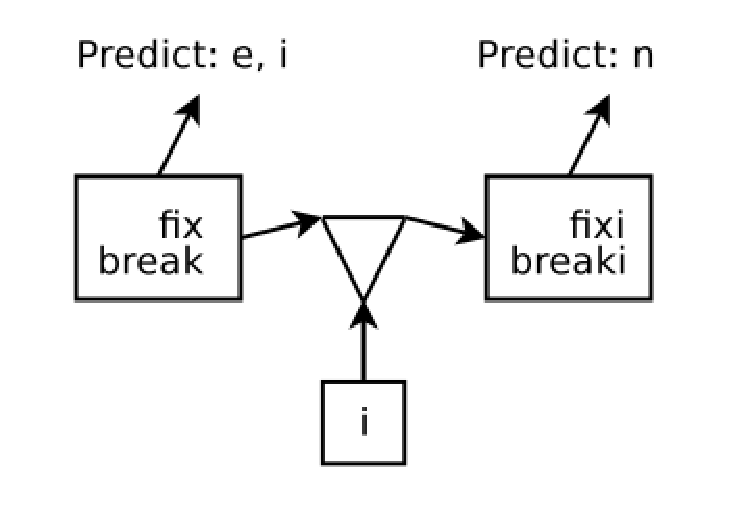
\includegraphics[width=.5\linewidth]{8_1_mrnn}\\
  \caption{A example that requires multiplicative connection}\label{fig:mrnn}
\end{figure}

For example in Figure \ref{fig:mrnn}, the character string ``ing'' is quite probable after ``fix'' and also quite probable after ``break''. If the hidden state vectors of the two words share a common concept of the stem of a verb, then there is a common representation to allow the character ``i'' to produce ``n''. Any evidence alone (verb stem or character ``i'') is not sufficient to make the prediction, and adding the weight additively is intuitively not a good strategy.

Based on the above analysis, in MRNN the update rule of hidden state vectors is changed to:
\begin{eqnarray}
h_t &=& tanh(W_{hx}x_t + W^{(x_t)}_{hh}h_{t-1} + b_h)
\end{eqnarray}
Here $W_{hh}$ is replaced with $W_{hh}^{(x_t)}$, allowing each character to specify a different hidden-to-hidden weight matrix.

The above scheme has a major drawback, which is that the storage required for $W_{hh}^{(x_t)}$ becomes prohibitive when the dimensionality of $x_t$ is even moderately large. The paper overcomes this problem by factoring $W_{hh}^{(x)}$ with three matrices $W_{fx}, W_{hf}$ and $W_{fh}$ \cite{Taylor2009Factored}:
\begin{eqnarray}
W_{hh}^{(x_t)} = W_{hf} \cdot diag(W_{fx}x_t) \cdot W_{fh}
\end{eqnarray}
As a result, the updating rules can be represented as:
\begin{eqnarray}
f_t &=& diag(W_{fx}x_t) \cdot W_{fh}h_{t-1}\\
h_t &=& tanh(W_{hf}f_t + W_{hx}x_t)\\
o_t &=& W_{oh}h_t + b_o
\end{eqnarray}

In the experimental section, the paper makes comparison study with the \emph{sequence memorizer}  and \emph{PAQ}  methods. It is reported that MRNN achieves lower \emph{bits per character (bpc)} than the sequence memorizer but higher than PAQ (lower bpc implies better performance). The second part of experiment is to evaluate different methods with the \emph{debagging problem}, which is to convert a bag of words into a meaningful sentence. MRNN recovers the correct ordering 34\% of the time, which is higher than the memorizer (27\% of the time). Finally and most interestingly, the proposed neural network is used to generate sentence in character level, given a beginning of the sentence. For example, when initialized with the phrase ``The meaning of life is'', the MRNN generates the following sentence:

\begin{small}
The meaning of life is the tradition of the ancient human reproduction: it is less favorable to the good boy for when to remove her bigger. In the show's agreement unanimously resurfaced. The wild pasteured with consistent street forests were incorporated by the 15th century BE. In 1996 the primary rapford undergoes an effort that the reserve conditioning, written into Jewish cities, sleepers to incorporate the .St Eurasia that activates the population. Mar??a Nationale, Kelli, Zedlat-Dukastoe, Florendon, Ptuos thought is. To adapt in most parts of North America, the dynamic fairy Dan please believes, the free speech are much related to the...
\end{small}


\section{Text-to-speech Synthesis} \label{Text-to-speech Synthesis}

The goal of the TTS component is to map a text to a waveform output. Speech synthesis systems typically perform this mapping in two steps, first converting the input text into a phonemic internal representation and then converting this internal representation into a waveform \cite{Jurafsky2006}.

We begin this section with a brief survey of the mature approach that are widely applied in commercial systems \cite{Jurafsky2006}. In the second paper, we introduce an end-to-end TTS system that works without explicit internal representation \cite{Wu2016Investigating}. This new line of research still awaits to be further explored, and is not among the mainstreams of commercial TTS systems.

\subsection{Speech Synthesis \cite{Jurafsky2014Speech}}

This section is a summary of Chapter 8, Speech Synthesis of the book Speech and Language Processing \cite{Jurafsky2014Speech}. In this summary we will see some main challenges and classic approaches of the \emph{text-to-speech (TTS)} task.

\begin{figure}[htbp]
  \centering
  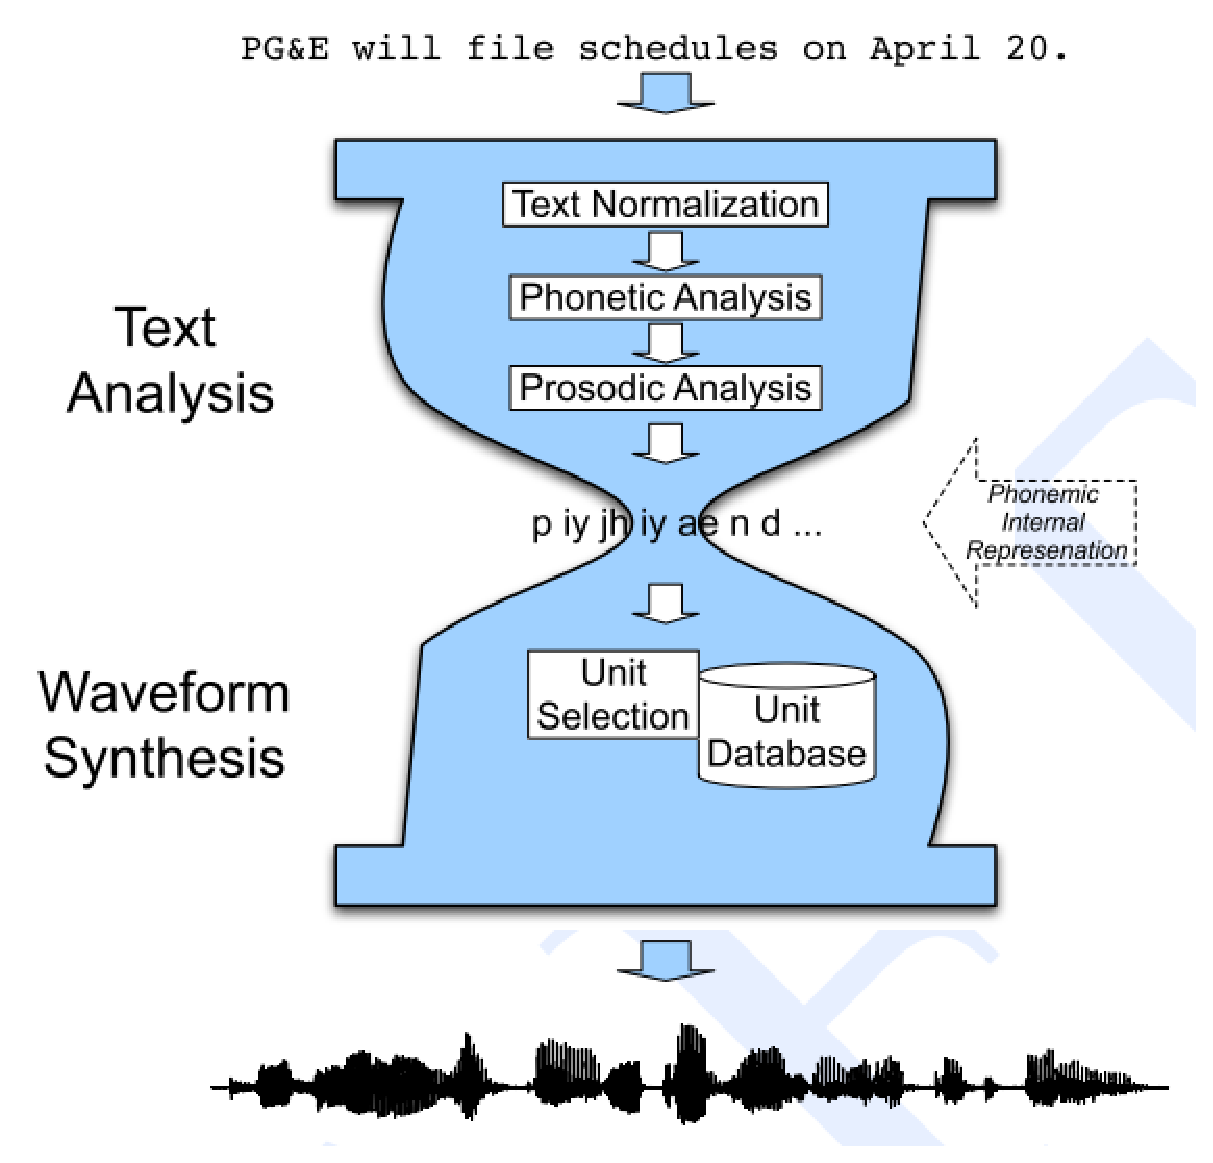
\includegraphics[width=.5\linewidth]{10_17_tts_arch}\\
  \caption{Architecture for the classic TTS system}\label{fig:TTS_arch}
\end{figure}

The goal of TTS is to map a text to a waveform output. The classic TTS architectures have two main steps, text analysis and waveform synthesis, as shown in Figure \ref{fig:TTS_arch}. While text analysis algorithms are relatively standard, there are three different paradigms for waveform synthesis: concatentative synthesis, formant synthesis and articulatory synthesis. Most modern commercial TTS systems are based on concatentative synthesis. Next we will explore each of the sub-tasks in further details.

The text analysis step has three main components: the text normalization component, the phonetic analysis component, and the prosodic analysis component. Each of them performs the following sub-tasks:
\begin{enumerate}
\item{Text Normalization:
    \begin{itemize}
    \item Sentence tokenization: This step segments a paragraph into a set of sentences, so that the TTS can synthesis speech for each sentence separately.
    \item Process non-standard words: There are several types of non-standard words, including numbers, abbreviations, acronyms and so on. For example, in `The European economy in 1750', the number 1750 is translated to `seventeen fifty'. But in `The password is 1750', the number should be translated to `one seven five zero'.
    \item Homograph disambiguation: Some words with the same spelling may have different pronunciations. For example, the word live in `live in China' should be pronounced differently from that in `a live animal'.
    \end{itemize}
}
\item{Phonetic Analysis: This stage takes the normalized word strings and produces a pronunciation for each word.
    \begin{itemize}
    \item Dictionary lookup: The first step is to directly lookup each word in the phonetic dictionary. For example, a sample entry in the CMU Pronouncing Dictionary is ``TABLE - T EY1 B AH0 L'' (0 denotes unstressed, 1 denotes stressed).
    \item Process names: There are many types of names, such as names of people, locations, organisations, etc. Some of the names may not appear in the dictionary. In the step the system need to decide how to pronounce them.
    \item Grapheme-to-phoneme: In this stage, the system uses letter-to-sound rules to process the remaining words.
    \end{itemize}
}
\item{Prosodic Analysis: The goal of the prosody analysis stage is to decide the rhythm, accent, stress, tune and other aspects of the speech.
    \begin{itemize}
    \item Prosodic structure: For example in a single phrase `I wanted to go to London', there seems to be some prosodic phrase boundaries that split up the words as follows: `I wanted | to go | to London'.
    \item Prosodic prominence: In any spoken utterance, some words sound more prominent than others. The notion of prominence is generally captured by a marker called pitch accent. The following example shows accented words in capital letters: `I'm a little SURPRISED to hear it.'
    \item Tune: A very obvious example of tune in English is the difference between statements and yes-no question. Consider the statement `you know what I mean' and the question `you know what I mean?'.
    \item Compute duration and F0 from prosodic labels: F0 refers to the lowest frequency of a complex wave. Some algorithms such as the unit selection synthesis approach do not need this step.
    \end{itemize}
}
\end{enumerate}

\begin{figure}[htbp]
  \centering
  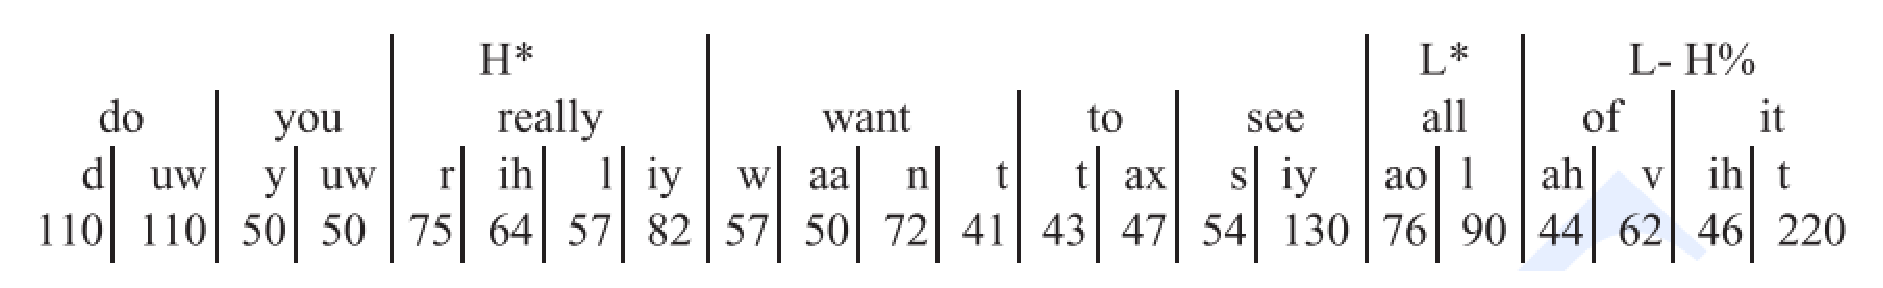
\includegraphics[width=.7\linewidth]{10_17_tts1}\\
  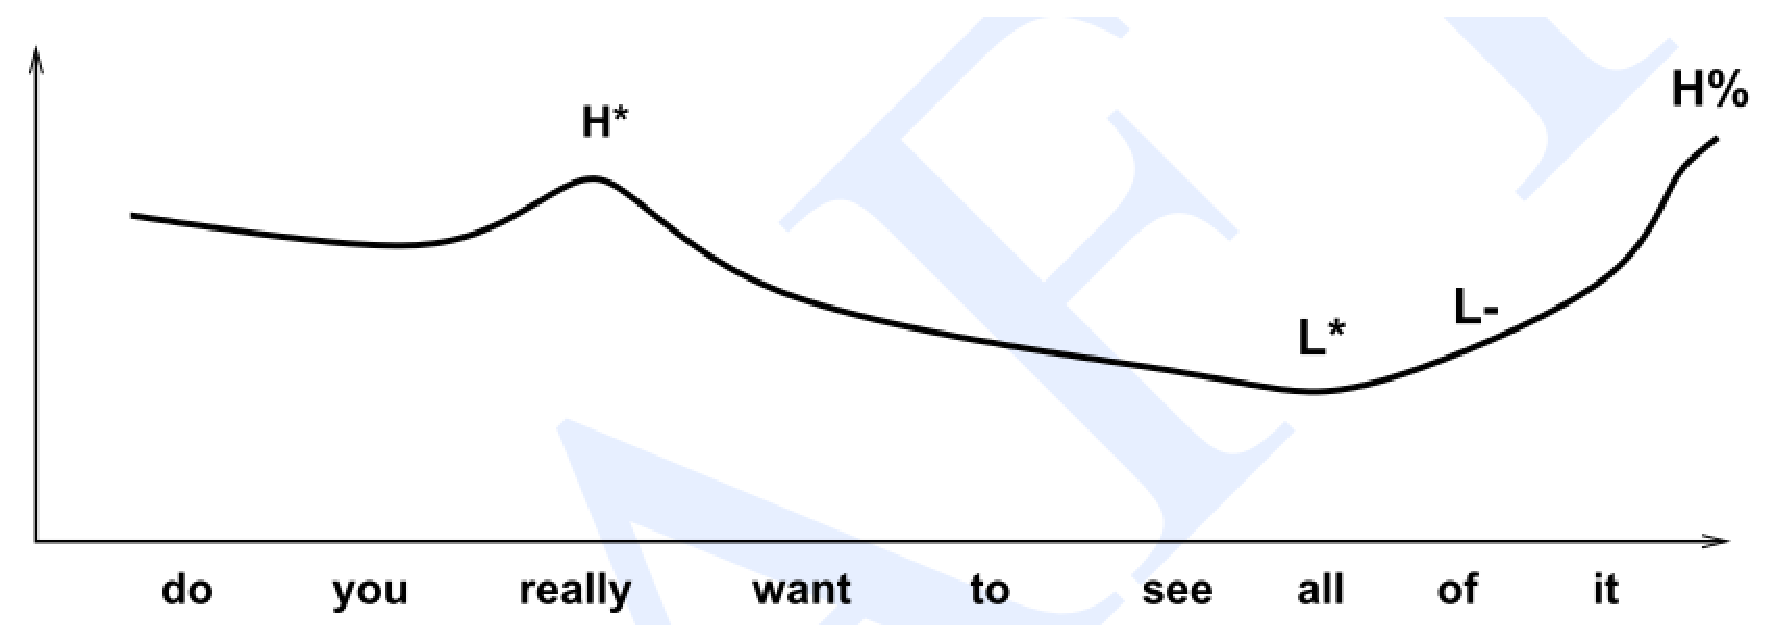
\includegraphics[width=.5\linewidth]{10_17_tts2}\\
  \caption{Internal representation of the FESTIVAL diphone system}\label{fig:TTS_inter}
\end{figure}

The final output of text analysis is called the internal representation of the input text sentence. Figure \ref{fig:TTS_inter} shows some TTS output from the FESTIVAL diphone system for the sentence `Do you really want to see all of it?'.

The next step is to turn the internal representation into a waveform. As aforementioned most of the modern commercial TTS systems are based on concatentative synthesis. The basic idea of concatentative approaches is to store the speech of human speakers in a database, and then retrieve and concatenate them according to the internal output. Two concatentative methods are discussed in this chapter: diphone synthesis and unit selection synthesis.

A diphone is a phone-like unit going from roughly the middle of one phone to the middle of the following phone. It takes a sequence of diphones from the database that corresponds to the desired phone sequence, and then concatenates them with some slight signal processing. Finally the algorithm performs some prosodic adjustments to the concatenated utterance.

Modern commercial TTS systems are based on a generalization of diphone synthesis, called unit selection synthesis. It differs from the classic diphone approach is two ways: 1) The unit selection database is much bigger (many hours long), containing many copies of each diphone; 2) Unit selection synthesis use no signal processing to the concatenated units, such as prosodic adjustments.

Finally, the section discusses some evaluation methods of the TTS systems. The development of a good automatic metric for speech synthesis remains an open question. Currently the speech synthesis systems are still evaluated by human listeners.

Remark: I think the TTS can be treated as an isolated component in our chatbot system. While it is intuitively beneficial to combine ASR and the dialogue manager (such as by jointly training), it seems difficult to improve TTS in a similar manner. I think we can use existing TTS system as a black box, without too much caring about how it works.

\subsection{Investigating gated recurrent networks for speech synthesis \cite{Wu2016Investigating}}

Recently, \emph{recurrent neural networks (RNNs)} have re-emerged as a potential acoustic model for \emph{statistical parametric speech synthesis (SPSS)}. This paper attempts to answer two questions: 1) why do LSTMs work well as a sequence model for SPSS; 2) which component of the LSTM unit is most important. It presents a visual analysis along the experiments, resulting in a simplified architecture.

The goal of the paper is to reach a better understanding of the ``black-box'' LSTM architecture. First, it gives an analysis of the forget gate and memory cell in the LSTM architecture. Specifically, it visualises the activation of the forget gate to understand when the forget gate resets the memory cell state, and how the forget gate relates to speech structure. Second, it analyses the importance of each LSTM component (e.g., input gate, output gate, forget gate), and proposes a simplified architecture.

To assess the importance of each component, the paper starts with four variants of the LSTM architecture: 1) No Peep-holes (NPH): Set the peep-hole connections $p^i, p^o, p^f$ to zeros. 2) No input gate (NIP): Set the input gate to 1 ($i_t = 1$). 3) No forget gate (NFG): Set the forget gate to 1 ($f_t = 1$). 4) No output gate (NOG):  Set the output gate to 1 ($o_t = 1$).

\begin{figure}[htbp]
  \centering
  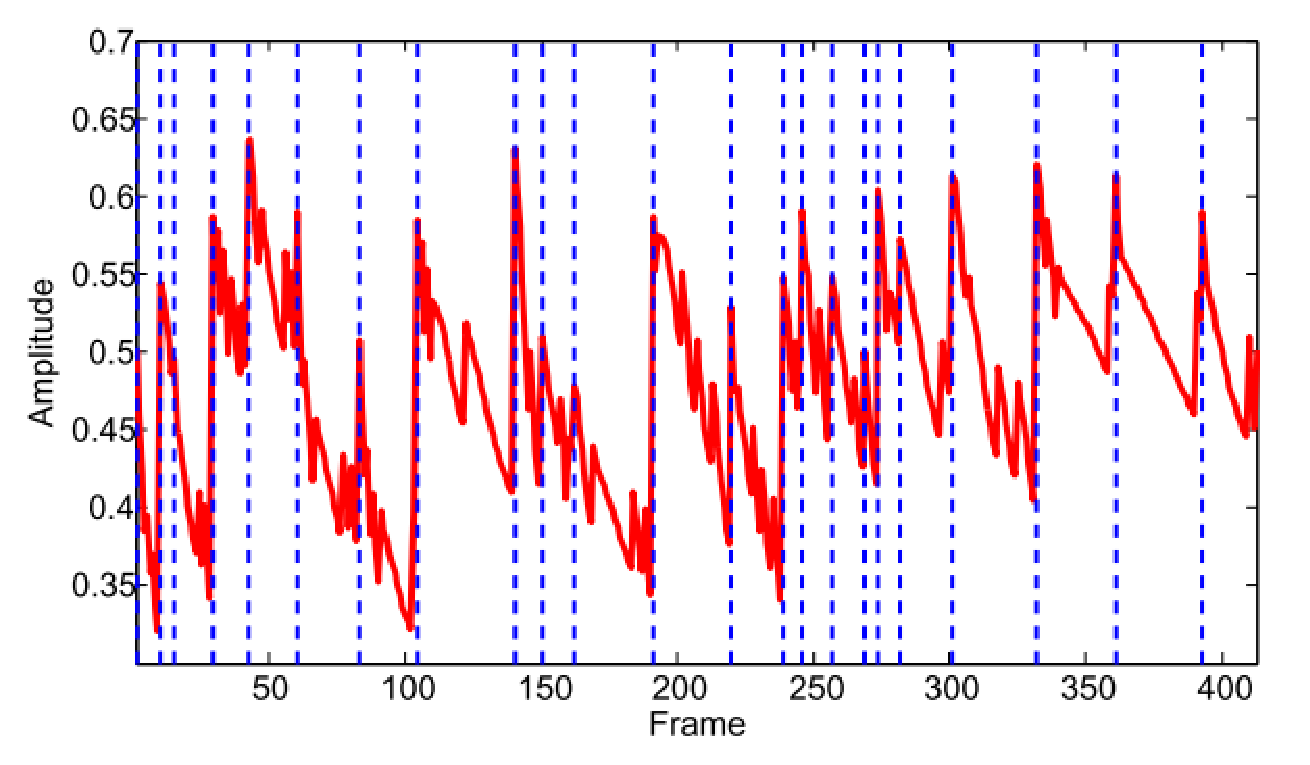
\includegraphics[width=.5\linewidth]{10_3_acu1}\\
  \caption{Averaged activations of all forget gates}\label{fig:acu1}
\end{figure}

\begin{figure}[htbp]
  \centering
  % Requires \usepackage{graphicx}
  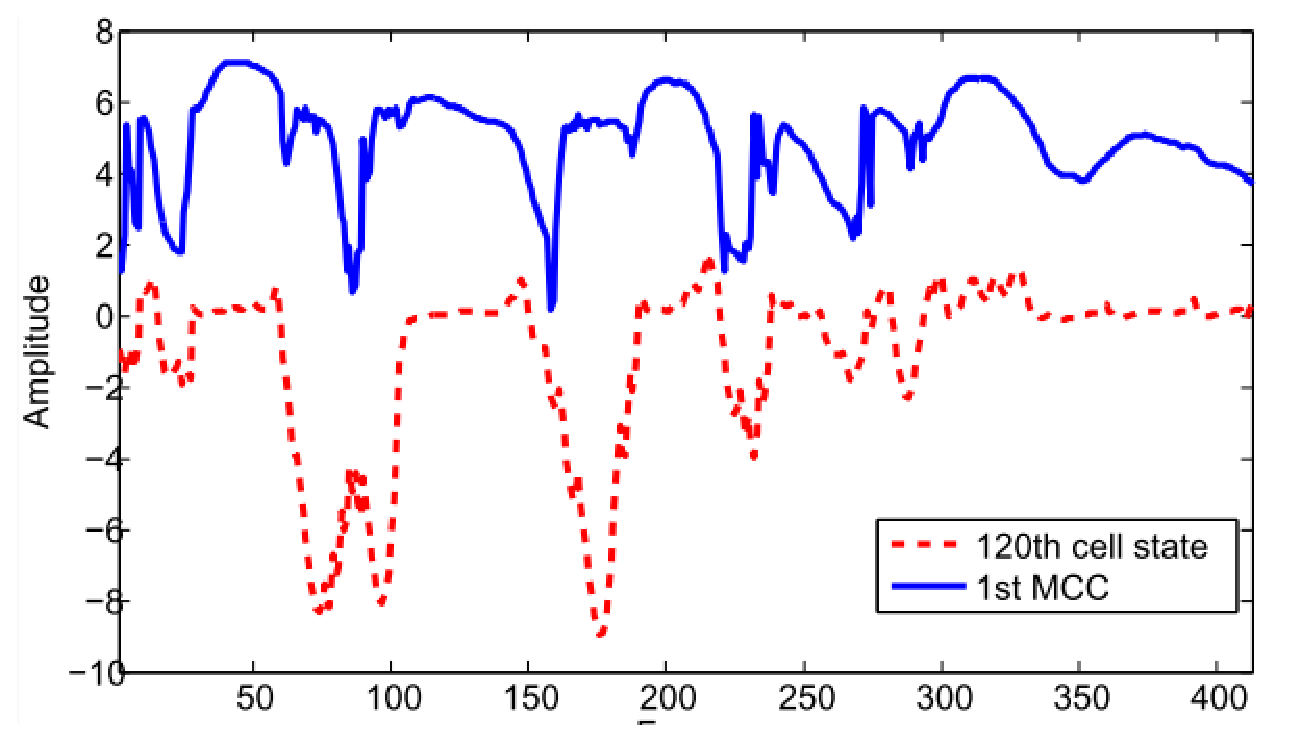
\includegraphics[width=.5\linewidth]{10_3_acu2}\\
  \caption{Comparison between the Mel-Cepstral Coefficient (MCC) trajectory and a cell state}\label{fig:acu2}
\end{figure}

The first step of the analysis is to visualise the forget gate and cell state, which are thought to be the two most important components in modelling long-term temporal structure. The averaged activations over the 256 units of the forget gate are presented in Figured \ref{fig:acu1}. It can be observed that the peaks of the forget gate activation trajectory have a strong correspondence with the phoneme boundaries. The memory cell should store the trend of the trajectory to be predicted, and a comparison between the relation is presented in Figure \ref{fig:acu2}.

The objective experiment compares the standard LSTM with different variations. The results show that the NFG system increases distortion considerably, which implies that the forget gate is the most important. Based on this observation, the paper proposes a simplified LSTM structure, which removes output gates and peep-hole connections, and replaces the input gate by the forget gate. The other experimental results also shows that the simplified LSTM is as good as any other systems.

Remark: This paper provides a detailed analysis of the performance of different components of the LSTM unit. In many occasions, we tend to use network architectures like LSTM as black boxs - we believe that they would work well because they are successful in other tasks. This paper reminds us that it is still necessary to look into why a network works on a specific problem. This may bring us deeper insight, and probably result in a better architecture.

\section{Non-goal-driven Systems} \label{Non-goal-driven Systems}

Non-goal-driven systems usually accomplish NLU, DM, and NLG jointly. Historically, they start as rule-based systems, such as ELIZA \cite{Weizenbaum1966Eliza} and ALICE \footnote{http://www.alicebot.org/}. As the amount of conversational corpus becomes large, data-driven systems have been researched since 2011 \cite{Ritter2011Data}. The methods used in data-driven systems fall into two categories: (1) Retrieval-based methods \cite{Ji2014An, Yan2016DocChat}; (2) Generation-based methods \cite{Ritter2011Data, Shang2015Neural, Sordoni2015Hierarchical, Serban2016Building}. Non-goal-driven systems may be useful for goal-oriented systems when they are trained on corpus related to the tasks of goal-oriented systems: (1) They can be used as user simulator to construct large task-specific corpus; (2) They may directly act as goal-oriented systems \cite{Vinyals2015A}.

\subsection{A neural conversational model \cite{Vinyals2015A}.}

The task is to build end-to-end trainable chatbots that can have multiple rounds of domain-specific or open-domain conversations. The paper applies sequence-to-sequence learning, which uses an encoder to map the input sequence to a fixed-length vector, i.e. the hidden state, and uses a decoder LSTM to decode the output sequence from the vector \cite{Sutskever2014Sequence}.

The encoder that is a multilayer LSTM takes a sequence of words ($x_{1},...,x_{T}$):
\begin{equation}
h_{t} \ = \ f( h_{t-1}, x_{t} ) \\
\end{equation}

Given the last hidden state of encoder, $h_{T}$, the decoder that is another multilayer LSTM computes the probability of generating next word:
\begin{equation}
\begin{aligned}
s_{t} \ =& \ f( s_{t-1}, y_{t-1}, h_{T} ) \\
y_{t} \ =& \ g( s_{t} )
\end{aligned}
\end{equation}
where $g$ is a softmax function. The encoder stops after generating a special end-of-sentence symbol EOS.

When trained on a domain-specific IT trouble shooting dataset, the chatbot can solve users' IT problems via multi-round conversations. When trained on an open-domain movie transcript dataset, the chatbot can remember facts and common sense knowledge, perform simple forms of reasoning, etc.

\subsection{Neural responding machine for short-text conversation \cite{Shang2015Neural}.}

The task is to build end-to-end trainable chatbots that can have one round conversations. The paper applies encoder-decoder framework, which uses GRU \cite{Chung2014Empirical, Cho2014Learning} encoders to encode the input post to a hidden state, and uses a GRU decoder to decode the output reply.

The encoders consist of a global encoder \cite{Chung2014Empirical, Cho2014Learning} and a local encoder \cite{Bahdanau2014Neural, Graves2013Generating}. The global encoder maps the input post to the last hidden state:
\begin{equation}
h_{t} \ = \ f( h_{t-1}, x_{t} ) \\
\end{equation}
where ($x_{1},...,x_{T}$) is a input sequence of words. The decoder uses $h_{T}$ as the context vector $c_{t}$

The local encoder maps the input post to weighted sum of hidden states when encoding the input post:
\begin{equation}
\begin{aligned}
h_{t} \ =& \ f( h_{t-1}, x_{t} ) \\
\alpha_{tj} \ =& \ q(s_{t-1}, h_{j}) \\
c_{t} \ =& \ \sum_{j=1}^{T} \alpha_{tj}h_{j} \\
\end{aligned}
\end{equation}

The decoder works as follows:
\begin{equation}
\begin{aligned}
s_{t} \ =& \ f( s_{t-1}, y_{t-1}, c_{t} ) \\
y_{t} \ =& \ g( s_{t} ) \\
\end{aligned}
\end{equation}


\subsection{Building end-to-end dialogue systems using generative hierarchical neural network models \cite{Serban2016Building}.}

The task is to build end-to-end trainable chatbots that can have open-domain conversations. The paper applies HRED \cite{Sordoni2015Hierarchical}, which uses encoder GRU \cite{Chung2014Empirical, Cho2014Learning} to encode the input utterance to an utterance vector, uses context GRU to map the utterance vector to a context vector, and uses decoder GRU to decode the context vector to generate the output response. The chatbots are improved by bootstrapping word embeddings from large news datasets with word2vec \cite{Mikolov2014Empirical}, or by pretraining model parameters on large QA datasets. The chatbots can also benefit from using bidirectional RNN \cite{Sundermeyer2014Translation}.

%%%%%%%%%%%%%%%%%%%%%%%%%%%%%%%%%%%%%%%%%%%%%%%%%%%%%%%%%%%%%%%%

\bibliographystyle{ieeetr}
%\bibliographystyle{model2-names}
\begin{thebibliography}{10}

\bibitem{Graves2013Generating}
Graves A. Generating sequences with recurrent neural networks. arXiv preprint, 2013.

\bibitem{Bahdanau2014Neural}
Bahdanau D., Cho K., Bengio Y. Neural machine translation by jointly learning to align and translate. ICLR, 2015.

\bibitem{Sutskever2014Sequence}
Sutskever I, Vinyals O, Le Q V. Sequence to sequence learning with neural networks. Advances in neural information processing systems, 2014.

\bibitem{Sundermeyer2014Translation}
Sundermeyer, M., Alkhouli, T., Wuebker, J., Ney, H. Translation Modeling with Bidirectional Recurrent Neural Networks. EMNLP 2014.

\bibitem{Mikolov2014Empirical}
Mikolov, T., Sutskever, I., Chen, K., Corrado, G. S., Dean, J. Distributed representations of words and phrases and their compositionality. Advances in neural information processing systems, 2013.

\bibitem{Cho2014Learning}
Cho, K., van Merrienboer, B., Gulcehre, C., Bougares, F., Schwenk, H., Bengio, Y.
Learning phrase representations using RNN encoder-decoder for statistical machine translation. Proceedings of the Empiricial Methods in Natural Language Processing, 2014.

\bibitem{Chung2014Empirical}
Chung, J., Gulcehre, C., Cho, K., Bengio, Y. Empirical evaluation of gated recurrent neural networks on sequence modeling. NIPS Deep Learning Workshop, 2014.

\bibitem{Wu2016Investigating}
Wu, Z., and King, S. Investigating gated recurrent networks for speech synthesis. In ICASSP 2016.

\bibitem{Young2013Pomdp}
Young, S., Gašić, M., Thomson, B., and Williams, J. D. Pomdp-based statistical spoken dialog systems: A review. Proceedings of the IEEE, 2013.

\bibitem{Levin2000A}
Levin, E., Pieraccini, R., and Eckert, W. A stochastic model of human-machine interaction for learning dialog strategies. IEEE Transactions on speech and audio processing, 2000.

\bibitem{Gašić2011Online}
Gašić, M., Jurčíček, F., Thomson, B., Yu, K., Young, S. On-line policy optimisation of spoken dialogue systems via live interaction with human subjects. ASRU, 2011.

\bibitem{Engel2014Reinforcement}
Engel, Y., Mannor, S., Meir, R. Reinforcement learning with Gaussian processes. In ICML, 2005.

\bibitem{Gašić2013Online}
Gašić, M., Breslin, C., Henderson, M., Kim, D., Szummer, M., Thomson, B., Tsiakoulis, P., Young, S. On-line policy optimisation of Bayesian spoken dialogue systems via human interaction. IEEE International Conference on Acoustics, Speech and Signal Processing, 2013.

\bibitem{Pascanu2012Understanding}
Pascanu R, Mikolov T, Bengio Y. Understanding the exploding gradient problem. CoRR, 2012.

\bibitem{Henderson2014Word}
Henderson, M., Thomson, B., Young, S. Word-based dialog state tracking with recurrent neural networks. In SIGDIAL, 2016.

\bibitem{Williams2016End}
Williams, J. D., and Zweig, G. End-to-end LSTM-based dialog control optimized with supervised and reinforcement learning. arXiv preprint, 2016.

\bibitem{Bordes2016Learning}
Bordes, A., Weston, J. Learning End-to-End Goal-Oriented Dialog. arXiv preprint, 2016.

\bibitem{Bengio2003A}
Bengio, Y., Ducharme, R., Vincent, P., and Jauvin, C. A neural probabilistic language model. Journal of Machine Learning Research, 2003.

\bibitem{Mahoney2005Adaptive}
Mahoney, M. V. Adaptive weighing of context models for lossless data compression. Technical Report, 2005.

\bibitem{Gasthaus2010Lossless}
Gasthaus, J., Wood, F., and Teh, Y. W. Lossless Compression Based on the Sequence Memoizer. In DCC, 2010.

\bibitem{Taylor2009Factored}
Taylor, G. W., and Hinton, G. E. Factored conditional restricted Boltzmann machines for modeling motion style. In ICML, 2009.

\bibitem{Sutskever2011Generating}
Sutskever, I., Martens, J., and Hinton, G. E. Generating text with recurrent neural networks. In ICML, 11.

\bibitem{Wen2015Stochastic}
Wen, T. H., Gasic, M., Kim, D., Mrksic, N., Su, P. H., Vandyke, D., Young, S. Stochastic language generation in dialogue using recurrent neural networks with convolutional sentence reranking. In SIGDIAL, 2015.

\bibitem{Sutton2010An}
Sutton, C., and McCallum, A. An introduction to conditional random fields. arXiv preprint, 2010.

\bibitem{Lafferty2001Conditional}
Lafferty, J., McCallum, A., and Pereira, F. Conditional random fields: Probabilistic models for segmenting and labeling sequence data. In ICML, 2001.

\bibitem{Finkel2005Incorporating}
Finkel, J. R., Grenager, T., and Manning, C. Incorporating non-local information into information extraction systems by gibbs sampling. In ACL, 2005.

\bibitem{Jurafsky2014Speech}
Jurafsky, D., and Martin, J. H. Speech and language processing. Pearson, 2014.

\bibitem{Graves2013Speech}
Graves, A., Mohamed, A. R., and Hinton, G. Speech recognition with deep recurrent neural networks. In IEEE international conference on acoustics, speech and signal processing, 2013.

\bibitem{Hinton2012Deep}
Hinton, G., Deng, L., Yu, D., Dahl, G. E., Mohamed, A. R., Jaitly, N., and Kingsbury, B. Deep neural networks for acoustic modeling in speech recognition: The shared views of four research groups. IEEE Signal Processing Magazine, 2012.

\bibitem{Rabiner1989A}
Rabiner, L. R. A tutorial on hidden Markov models and selected applications in speech recognition. Proceedings of the IEEE, 1989.

\bibitem{Vinyals2015A}
Vinyals, O. and Le, Q. A neural conversational model. arXiv preprint, 2015.

\bibitem{Serban2016Building}
Serban, I. V., Sordoni, A., Bengio, Y., Courville, A., Pineau, J. Building end-to-end dialogue systems using generative hierarchical neural network models. AAAI, 2016.

\bibitem{Sordoni2015Hierarchical}
Sordoni, A., Bengio, Y., Vahabi, H., Lioma, C., Grue Simonsen, J., Nie, J. Y. A hierarchical recurrent encoder-decoder for generative context-aware query suggestion. CIKM, 2015.

\bibitem{Shang2015Neural}
Shang L, Lu Z, Li H. Neural responding machine for short-text conversation. EMNLP, 2015.

\bibitem{Yan2016DocChat}
Yan, Z., Duan, N., Bao, J., Chen, P., Zhou, M., Li, Z. and Zhou, J., DocChat: An Information Retrieval Approach for Chatbot Engines Using Unstructured Documents. In ACL, 2016.

\bibitem{Ji2014An}
Ji Z, Lu Z, Li H. An information retrieval approach to short text conversation. arXiv preprint, 2014.

\bibitem{Ritter2011Data}
Ritter, A., Cherry, C., and Dolan, W. B. Data-driven response generation in social media. In Proceedings of the conference on empirical methods in natural language processing, 2011.

\bibitem{Weizenbaum1966Eliza}
Weizenbaum, J. ELIZA - a computer program for the study of natural language communication between man and machine. Communications of the ACM, 1966.

\end{thebibliography}

\bibliography{d:/research/chatbot}

\end{document}
